\documentclass[12pt]{article}
\usepackage[top=1in, bottom= 1in, left= 1in, right= 1in]{geometry}
\usepackage[USenglish]{babel}
\usepackage{natbib}
\usepackage{multirow}
\usepackage{graphicx, subfigure}
\usepackage{fancyhdr}
\usepackage{setspace}
\usepackage{verbatim}
\usepackage{booktabs}
\usepackage{amsmath}
\usepackage{lscape}
\usepackage{dcolumn}
\usepackage{floatrow}
\usepackage[title]{appendix}
\usepackage{xcolor}
\usepackage{todonotes}
\usepackage[colorlinks=true,citecolor=red!50!black,urlcolor=blue!50!black,linkcolor=red!50!black]{hyperref}
\setlength{\headheight}{15pt}

\author{Patrick W. Kraft\footnote{Ph.D. Student, Stony Brook University, \href{mailto:patrick.kraft@stonybrook.edu}{patrick.kraft@stonybrook.edu}.
%I thank Stanley Feldman, Jennifer Jerit, Scott Clifford, Peter DeScioli, Jason Barabas, and participants of the Political Science Graduate Student Colloquium at Stony Brook University as well as the participants at the panel of the 2015 Annual Meeting of the Midwest Political Science Association for helpful comments on earlier versions of this draft.
}}
\date{today}

\title{Moral Foundations of Political Reasoning\footnote{An earlier version of this paper was presented at the 73rd Annual Conference of the Midwest Political Science Association, April 16-19, 2015. The manuscript and code are available on GitHub: \url{https://github.com/pwkraft/mft}.}\\
\large{Investigating the Moral Underpinnings of Political Judgment}}
\date{\today}


\begin{document}
\maketitle
\onehalfspacing

\begin{abstract}
The goal of this paper is to investigate whether and how individuals rely on moral foundations when evaluating political candidates and parties. Based on open-ended survey responses in the 2008 and 2012 American National Election Study, it will be examined whether differences in moral judgments between liberals and conservatives shape and structure individual reasoning and evaluations in the political context. More specifically, I utilize the moral word lists to identify references to basic moral intuitions when individuals report on their attitudes towards political parties and candidates. It can be shown that liberals and conservatives differ with regard to the set of moral foundations they rely on when evaluating political actors. Furthermore, I find that the emphasis on specific moral considerations in political evaluations predicts voting behavior even after controlling for political predispositions. However, ideological differences in moral reasoning appear to be context-specific and are not always consistent with theoretical expectations of Moral Foundations Theory.

\vspace{\baselineskip}
\noindent \textbf{Keywords:} Moral Foundations Theory, Political Ideology, Political Reasoning, Open-ended Survey Responses
\end{abstract}
\newpage

\section{Introduction}

There has been a marked increase in political polarization and partisan sorting in the American public \citep{abramowitz2013polarized,levendusky2009partisan}. Recent studies that conceive of partisanship as a social identity show that partisanship elicits more extreme evaluations and behavioral responses to ingroups and outgroups than race \citep[e.g.][]{iyengar2014fear}, and that hostility across party lines has been growing for decades \citep{haidt2012look,iyengar2012affect}. The source of this chasm, however, is less clear. Why do partisans seem to disagree so sharply about politics?  One answer to this puzzle may lie in the moral views of opposing partisans. Indeed, if one looks at the content of recent political debates, many polarized issues become a question of morality. Common examples include issues like abortion and same-sex marriage. However, it has been shown that even for issues that are not immediately conceived as intrinsically ``moral'', strong partisans not only disagree based on policy-based considerations, but they also view certain positions as morally right or wrong \citep{skitka2005moral,skitka2010psychology,ryan2014reconsidering}. The purpose of this study is to examine whether liberals and conservatives exhibit systematic differences in the moral considerations they bring to bear in day-to-day political reasoning as well as the consequences for political behavior.

Moral foundations theory describes five central innate intuitions that structure moral thinking \citep{haidt2008moral}. There is evidence that liberals and conservatives rely on different configurations of five “moral foundations” \citep{graham2009liberals}, and that a person’s endorsement of these foundations is related to vote choice \citep{iyer2010beyond} and preferences regarding many culture war issues \citet{koleva2012tracing}. Yet, most of this work relies on closed-ended questions that ask people to make judgements of moral relevance \citep{clifford2015moral}. However, most empirical investigations in this area rely on explicit ratings of abstract moral principles. As such, \citet[1031]{graham2009liberals} describe reports on moral relevance, which are part of the Moral Foundations Questionnaire, as ``self-theories of moral judgment'', rather than direct measures of judgment itself. \citet{clifford2015moral} addressed this issue by proposing as set of moral foundations vignettes, which measure actual moral judgment in scenarios more directly. The extent to which people draw upon the moral foundations in day-to-day political reasoning--without being explicitly asked about moral considerations--remains an open question. The paper presented here complements this effort of improving the measurement of moral reasoning by focusing on the conditions under which latent differences in moral foundations between liberals and conservatives manifest themselves in the political realm when the issue of morality is not explicitly raised.

% cite iyer here?
% Here you have a succinct statement of your critique of existing measure. I just took a stab at this; you can probably do better.  Right now this para feels too short to me—trying to cover too much ground.  You can try to improve it.

The present study complements previous research by investigating patterns of moral reasoning among individuals in a more unobtrusive survey context, where the potential connection between morality and politics is not induced or facilitated by design.

% Here you describe your different measurement strategy and why it is an improvement

Therefore, the goal of this paper is to investigate whether individuals rely on moral foundations when evaluating political candidates and parties without explicitly being asked about moral considerations. Accordingly, it will be examined whether the apparent differences in moral judgments between liberals and conservatives actually shape and structure individual reasoning and evaluations in the political context. The analyses are based on open-ended survey responses in the 2012 American National Election Study. More specifically, I utilize the moral word lists used by \citet{graham2009liberals} to identify references to basic moral intuitions when individuals report on their attitudes towards political parties and candidates.

Using the moral word lists developed by \citet{graham2009liberals}, I examine whether people reference the moral foundations when reporting their attitudes towards political parties and candidates in the open-ended likes-dislikes questions in the 2008 and 2012 American National Election Study. Overall, the results indicate that liberals and conservatives differ in their reliance on different moral considerations. However, these differences are not always consistent with theoretical expectations of Moral Foundations Theory and they also appear to be more contingent in that they are moderated by political expertise, media exposure, and political discussions. 

% Maybe end with a line or two about the implications of your findings. This may be a bit too short, and clearly still needs some work. But I really urge you to compose an intro section that is no more than 2 pages long.


\section{Theoretical Framework}

%A growing body of literature in political science and psychology investigates basic individual characteristics and underlying motivations that shape political belief systems and ideologies \citep[c.f.][]{jost2003political,jost2006end,jost2009political}. For example, it has been shown that liberals and conservatives differ with regard to their personality \citep{gerber2010personality,hirsh2010compassionate,de2013personality}, social values \citep{schwartz2010basic,schwartz2011basic,piurko2011basic}, or moral considerations \citep{lakoff1995metaphor,haidt2008moral,mcadams2008family}.

%Do can these systematic differences in individual emphasis on moral foundations explain growing disagreements between partisans? Haidt and colleagues argued that different moral considerations can reinforce disagreements in the political realm since liberals and conservatives base their judgments and arguments ``on different configurations of the five foundations'' \citep[1040]{graham2009liberals}.

%Consistent with \citet{graham2009liberals}, it is hypothesized that liberals and conservatives differ with regard to the set of moral foundations they rely on when evaluating political actors. However, \citet{graham2009liberals} stated that the causal nature of this relationship is not yet established. More specifically, their study did not settle whether individuals first identify as liberal or conservative and then adapt their respective moral judgments, or whether moral considerations shape and structure subsequent ideological thinking itself. Recent research focusing on elite influences on moral reasoning suggests that political elite rhetoric plays an important role in shaping individual moral judgment, which indicates that the influence of moral judgments in politics is indeed context-specific \citep[see for example][]{clifford2013words,clifford2015concerns}.



\subsection{Moral Foundations Theory}

In one of his influential earlier works on moral psychology, \citet{haidt2001emotional} argued that moral judgment is not based rational reasoning but rather on automatic and affective intuitions, which are in turn influenced by social and environmental factors. More specifically, \citet[825]{haidt2001emotional} described that moral intuition ``appears to be the automatic output of an underlying, largely unconscious set of interlinked moral concepts. These concepts may have some innate basis [...], which is then built up largely by metaphorical extensions from physical experience''. According to this view, explicit moral reasoning can then be better described as a rationalization of these intuitions. \citet{haidt2004intuitive} further developed this view of innateness as a framework to explain cultural differences in moral virtues.

As such, one of the major arguments in the framework of Moral Foundations Theory is the proposition that morality is partially innate, which \citet[367]{haidt2008moral} described as ``organized, to some extent, in advance of experience'' \citep[but see][]{suhler2011can}. More specifically, \citet{haidt2008moral} identified five basic intuitions which build the psychological foundations of human morality and are inherently linked to evolutionary adaptive challenges that appear cross-culturally. These five basic intuitions are \textit{Harm/Care}, \textit{Fairness/Reciprocity}, \textit{Ingroup/Loyalty}, \textit{Authority/Respect}, and \textit{Purity/Sanctity} \citep[see also][]{graham2011mapping}.\footnote{It is worth noting that later accounts of Moral Foundations Theory discussed the inclusion of further dimensions, such as \textit{Liberty/Oppression} \citep[c.f.][]{graham2013moral,haidt2012righteous}. However, the analyses presented here will only focus on the dimensions initially suggested in \citet{haidt2008moral}.} They represent an innate draft of morality that is further edited by individual experience. This editing process, in turn, is determined by the development of moral virtues as personal characteristics as well as moral narratives \citep{haidt2008moral}.

Numerous research has shown that this theoretical framework provides useful insights into the underlying factors shaping political belief systems and ideologies. As such, we now turn to the discussion of the relationship between moral values and political ideologies.


\subsection{Moral Values and Political Ideology}

Moral and social values have been described as one of the underlying personal characteristics that determine broader political beliefs. For example, \citet{piurko2011basic} described how basic personal values structured underlying motivational meanings of liberal and conservative political orientations \citep[see also][]{schwartz2010basic,schwartz2011basic}. Focusing more closely on moral values, \citet{lakoff1995metaphor} argued that conservative and liberal belief systems can be differentiated by their relative emphasis on specific moral metaphors, namely the strict father model as well as the nurturant parent model. In a subsequent study, \citet{barker2006competing} showed that these nurturant and disciplinarian visions of parental roles can indeed be connected to ideologically coherent views.

As such, the possible connection between moral values and political belief systems also became a major focus in the context of the Moral Foundations framework \citep[c.f.][]{haidt2012righteous}. \citet{haidt2007morality} as well as \citet{graham2009liberals} argued that liberal morals focus on individualizing foundations, which include harm/care and fairness/reciprocity. Conservatives, on the other hand, also emphasize the remaining foundations of ingroup/loyalty, authority/respect, and purity/sanctity, which are labelled as binding foundations. One interesting aspect about their expectations as well as their empirical results is that conservatives do not prioritize less on the individualizing foundations than liberals, but rather that liberals differ in their lower degree of emphasis on binding foundations. Compared to liberals, conservatives tend to endorse and use the five foundations more equally.

\citet{graham2009liberals} presented several empirical analyses to support their hypothesis. More specifically, the authors demonstrated that liberals showed greater endorsement and use of harm/care and fairness/reciprocity foundations when they were asked to evaluate the relevance of moral concerns, when they made explicit moral judgments, as well as in the context of moral trade-offs. Throughout these studies, conservatives endorsed and used the five foundations more equally. The final study presented by \citet{graham2009liberals} consisted of a quantitative analysis of sermons from liberal and conservative churches. The authors proposed a dictionary of words (and word stems) that signal references to the specific moral foundations and showed that liberal sermons where more likely to contain expressions that can be ascribed to the moral foundations of harm/care and fairness/reciprocity. As will be further described below, the analyses presented here will utilize the same dictionary in order to assess moral references in the context of open-ended survey responses.

Overall, these studies strongly support the view that the underlying moral intuitions conceptualized in the Moral Foundations framework differ systematically between liberals and conservatives. While subsequent studies looked more closely at the relationship between moral intuitions and multi-dimensional conceptualizations of ideology \citep[c.f.][]{haidt2009above}, as well as more specific sociopolitical orientations such as social dominance orientation and right-wing authoritarianism \citep[c.f.][]{federico2013mapping}, we will now turn to the question under what conditions the connection between moral values and political ideology manifests itself when citizens reason about politics and evaluate political actors.


\subsection{The Role of Political Reasoning and Sophistication}

While the research discussed above convincingly showed that liberals and conservatives indeed show different patterns in their emphasis on moral foundations, it is still worth investigating whether these considerations differentiate how individuals reason about politics. Indeed, \citet{haidt2008moral} emphasized the importance of moral narratives in the development of moral thinking and \citet{mcadams2008family} showed how conservatives and liberals differed in terms of moral references in life-narrative interviews. But do these moral narratives also shape citizens' political evaluations and reasoning?

Looking at research on political attitudes and behavior from different perspectives suggests that this is indeed the case. For example, using open-ended survey responses in the context of social welfare attitudes, \citet{feldman1992political} showed that most people make references to values when they discuss their policy preferences. Looking at the elite level, \citet{clifford2013words} argued that proponents and opponents of stem cell research place distinctive weights on moral foundations which in turn affected the public attitudes and the underlying considerations related to the issue. Furthermore, \citet{clifford2014linking} presented a theory that suggests that individuals rely on their own moral motivations in order to interpret and evaluate the behavior of politicians. \citet{marietta2007values} also argued that political value priorities can serve as heuristics for electoral decision-making.
% para undercuts claim of novelty, make it sound like we already know the answer

Accordingly, numerous evidence suggests that moral foundations play an important role in the political debate as well as in the evaluation of political actors. Taking into account the fact that moral intuitions (or values in general) appear to play an important role on the elite as well as the electoral level suggests, that citizens can be expected to rely on references to moral foundations when reporting on their attitudes towards political actors. Consistent with the arguments and empirical evidence presented by \citet{graham2009liberals} and others, the following hypothesis can be specified:

\vspace{0.3cm}
\begin{tabular}{lp{12cm}}
\textsl{Hypothesis 1:} & Liberals are more likely to emphasize moral foundations of harm/care and fairness/reciprocity  than conservatives when evaluating political parties and candidates in the context of open-ended survey items. On the other hand, conservatives are more likely to emphasize moral foundations of ingroup/loyalty, authority/respect, and purity/sanctity than liberals.
\end{tabular}
\vspace{0.5cm}

However, the extent to which individuals rely on moral considerations when evaluating political actors cannot be expected to be universal among individuals and accross contexts. Rather, the general tendency to emphasize moral foundations is contingent upon individual levels of political sophistication, media exposure, and political discussions \citep[see also][]{goren2001core,goren2004political}. For example, \citet{clifford2015concerns} shows that elite rhetoric plays an important role in linking individual moral foundations with political attitudes. Accordingly, the following additional hypothesis can be specified:

%
% THIS ARGUMENT NEEDS TO BE STRONGER
%

\vspace{0.3cm}
\begin{tabular}{lp{12cm}}
\textsl{Hypothesis 2:} & Individuals who have more experience and are more engaged in the political system (i.e. with higher political sophistication, high media exposure, frequent political discussions, prior participation) are more likely to emphasize moral foundations when evaluating political parties and candidates.
\end{tabular}
\vspace{0.5cm}

Moral Foundations Theory proposes that innate differences in the emphasis of moral considerations provide the basis for diversity in ideological and political reasoning. However, the hypothesis outlined above suggestes that moral reasoning could also be viewed as a rhetorical tool that citizens use in order to support their preferences and bolster their views in front of others. If the emphasis on moral considerations is indeed contingent upon political engagement, exposure to political media, and frequent discussions, it suggests that moral reasoning can be viewed as a learning process in a polarized political environment. The following section will now present the empirical analyses conducted to test these hypotheses.


\section{Empirical Analyses}

\subsection{Data, Variables, and Model Specification}

The analyses presented here are based on the 2008 and 2012 American National Election Study. While the 2008 ANES consists of a single representative cross-sectional sample, the 2012 study contains two representative cross-sectional samples. One sample was conducted by computer assisted face-to-face interviews while the other sample is based on an internet panel group. Both samples are pooled in the analyses. While both samples consisted of a pre-election and a post-election wave, most items described below are drawn from the pre-election wave.\footnote{The main reason to focus on the pre-election wave is the fact that the open-ended items were only conducted prior to election day. Accordingly, wherever possible, the set of explanatory variables was also limited to those collected at the same time.}

As already indicated above, the major dependent variables are based on open-ended questions where respondents were asked to report which aspects they \textit{liked} and \textit{disliked} about either presidential candidate as well as the Republican and Democratic party in general. More specifically, respondents where asked to list anything in particular that they like/dislike about the Democratic/Republican party as well as anything that might make them vote/not vote for either of the Presidential candidates and were probed by the interviewer asking ``anything else?'' until the respondent answered no.

Using open-ended questions instead of closed survey responses has important advantages in the context of the research question proposed here. As described above, the studies by \citet{graham2009liberals}, which focused on self-reported moral judgments, convincingly demonstrated systematic patterns of moral reasoning that allowed to differentiate between liberals and conservatives. However, since moral considerations and political beliefs were measured explicitly using closed items, it could be argued that these associations are only latent and do not necessarily manifest themselves in actual day-to-day political reasoning. As mentioned above, self-reports on moral relevance do not necessarily describe how actual moral jugments are made (c.f. \citealt[1031]{graham2009liberals}, see also \citealt{clifford2015moral}). The paper presented here tries to contribute to previous efforts by investigating patterns of moral reasoning among individuals in a more unobtrusive survey context, where the potential connection between morality and politics is not induced or facilitated by design. When answering general open-ended survey responses on likes and dislikes about either parties and candidates, respondents can \textit{decide} to talk about moral considerations (without explicitly being asked to do so), rather than explicitly asked to make moral judgments. Finding similar patterns in such a context provides much stronger evidence for the notion that political reasoning is directly influenced by basic moral intuitions.

All survey responses were preprocessed by correcting spelling errors using an implementation of the Aspell spell checking algorithm in \texttt{R} (\url{www.aspell.net}). Furthermore, all individuals who responded in Spanish were deleted. Subsequently, it was examined whether the responses contained any of the signal words (or word stems) for each of the moral foundations as specified in the dictionary proposed by \citet{graham2009liberals}. This analyses was conducted using automatic word (stem) matching procedures in \texttt{R}. The specific word lists are also presented in Appendix A. 

For example, words like ``protect'' and ``suffer'' indicate references to the harm/care foundation, ``equality'' and ``tolerant'' signal reasoning based on the fairness/reciptocity foundation, ``patriot'' and ``betrayal'' indicate reference to the ingroup/loyalty foundation, ``honor'' and ``respect'' signal considerations related to authority/respect, whereas ``integrity'' and ``duty'' indicate reference to the purity/sanctity foundation.

After counting the occurrence of any of the signal words, the responses to the open-ended items (likes/dislikes for either parties and candidates) were collapsed since many of the respondents did not provide answers to every single one of them. Accordingly, the data used in the analyses described below consist of a matrix of dichotomous variables which indicate whether each respondent mentioned either of the five moral foundations in \textit{any} of the open-ended responses. If participants failed to provide an answer in any of the items, the variable for each moral foundation is specified as missing.

Table~\ref{tab:a1_mis} in the Appendix provides an overview over the number of omitted cases due to the fact that respondents did not provide responses to any of the items, or for which the interview language was Spanish. About 4\% of the interviews were held in Spanish in both surveys. Furthermore, about 7\% of the respondents in both datasets did not provide any open-ended responses. However, these proportions are much larger if we only take into account either open-ended candidate evaluations (13-14\%), or open-ended party evaluations (25\%). Furthermore, Figure~\ref{fig:a0_num} in the appendix displays histograms of the length of the respondents' answers to all open-ended items (i.e. summed over all responses), as well for candidate and party evaluations separately.

Since the individual response patterns are non-exclusive in the sense that individuals can (and do) mention more than one of the moral foundations in their answers, it is not possible to model them in a multinomial logit or conditional logit framework. While such an approach would come with the benefit of estimating a unified model for the overall response pattern, it does not allow for instances where single observations are able to select several alternatives \citep[but see][]{gilbert2007models}. Therefore, individual response patterns are modeled as independent dichotomous outcomes via logistic regressions for each of the moral foundations under consideration \citep[c.f. for example][]{agresti1999modeling}.

The major independent variable used to predict the individual likelihood to mention either of the moral foundations, is \textit{political ideology}. Respondents were asked to place themselves on a seven-point scale ranging from extremely liberal to extremely conservative. Since there are no clear theoretical reasons to suggest a priori that moderates should fall in between liberals and conservatives in terms of their moral foundations (i.e. that the relationship between `continuous' ideological self-placement and the likelihood to mention specific moral foundations is inherently linear), I constructed dichotomous variables indicating whether respondent identified as liberals, conservatives, or moderates.

The second set of independent variables under consideration as predictors of references to moral foundations in general include \textit{political sophistication}, which was measured as the sum of knowledge questions for which respondents provided correct responses. Since the 2008 ANES did not contain such items, political knowledge was measured as a dummy indicating whether respondents were able to identify the Republican party as more conservative than the Democratic party. Furthermore, the analyses investigate the effect of \textit{political media exposure} as well as the frequency of \textit{political discussions} with friends and family members. Further control variables included in the analyses are \textit{church attendance}, \textit{education} (college degree), \textit{age}, \textit{sex}, as well as \textit{race} (African American). Some supplemental analyses also include measures of \textit{party identification} which were constructed similarly to the conceptualization of political ideology.


\subsection{Results}

\subsubsection{Ideological Differences in Moral Reasoning}

\begin{figure}[ht]\centering
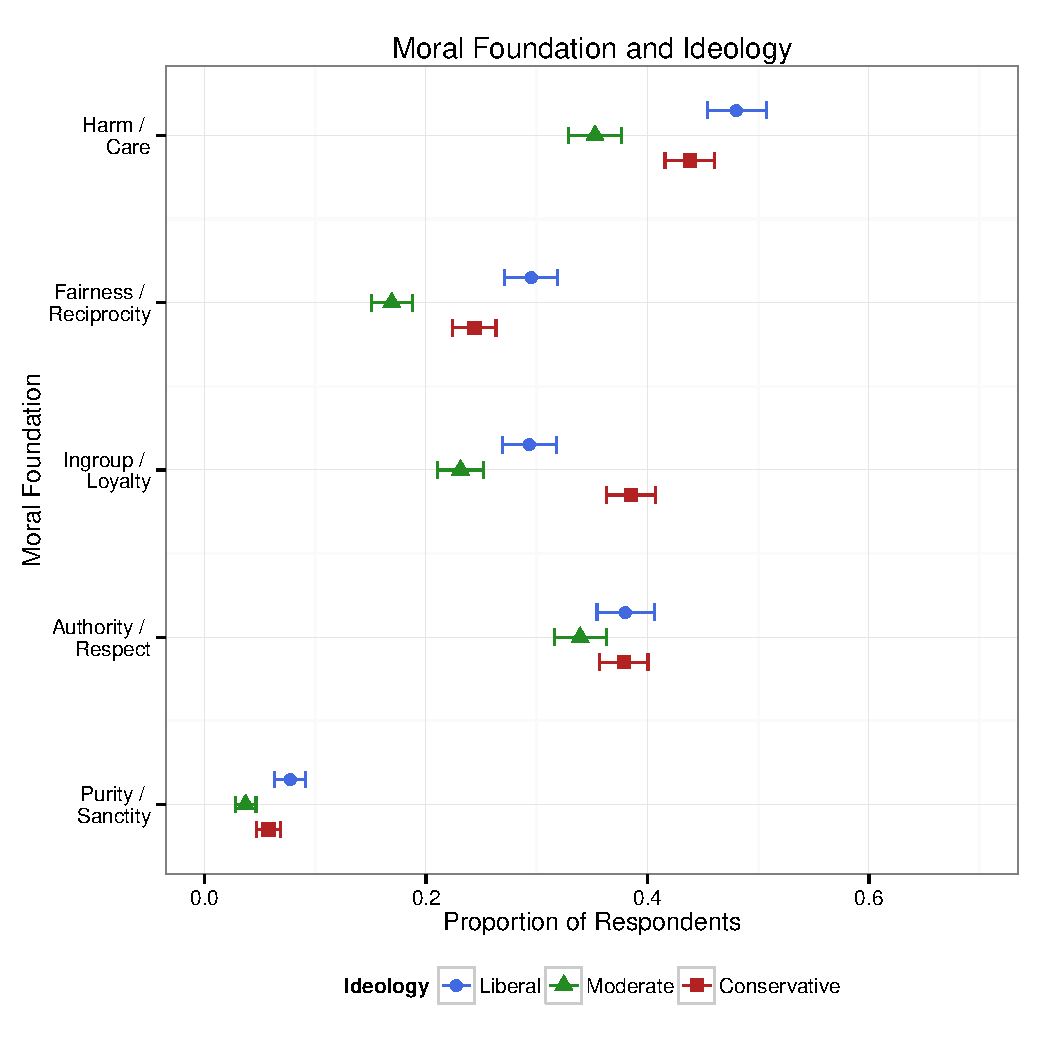
\includegraphics[scale=.6]{../calc/fig/p1_mft_ideol.pdf}
\caption{Moral Foundations and Ideology (all Statements)}\label{fig:mft_ideol}
\end{figure}

Before discussing the actual model estimates, Figure~\ref{fig:mft_ideol} provides an overview over the response patterns for individuals who identified as liberals, conservatives, or moderates. For each group, the Figure displays the proportion of respondents who mentioned words that were included in the five different moral foundations dictionaries as well as their 95\% confidence intervals. In order to calculate these proportions, all responses to the eight open-ended like/dislike questions (evaluating both parties and both candidates) were aggregated for each individual. Therefore, each proportion indicates the percentage of individuals who mentioned a signal word belonging to the respective moral foundation in any of his or her open-ended responses evaluating the parties or candidates.

\begin{figure}\centering
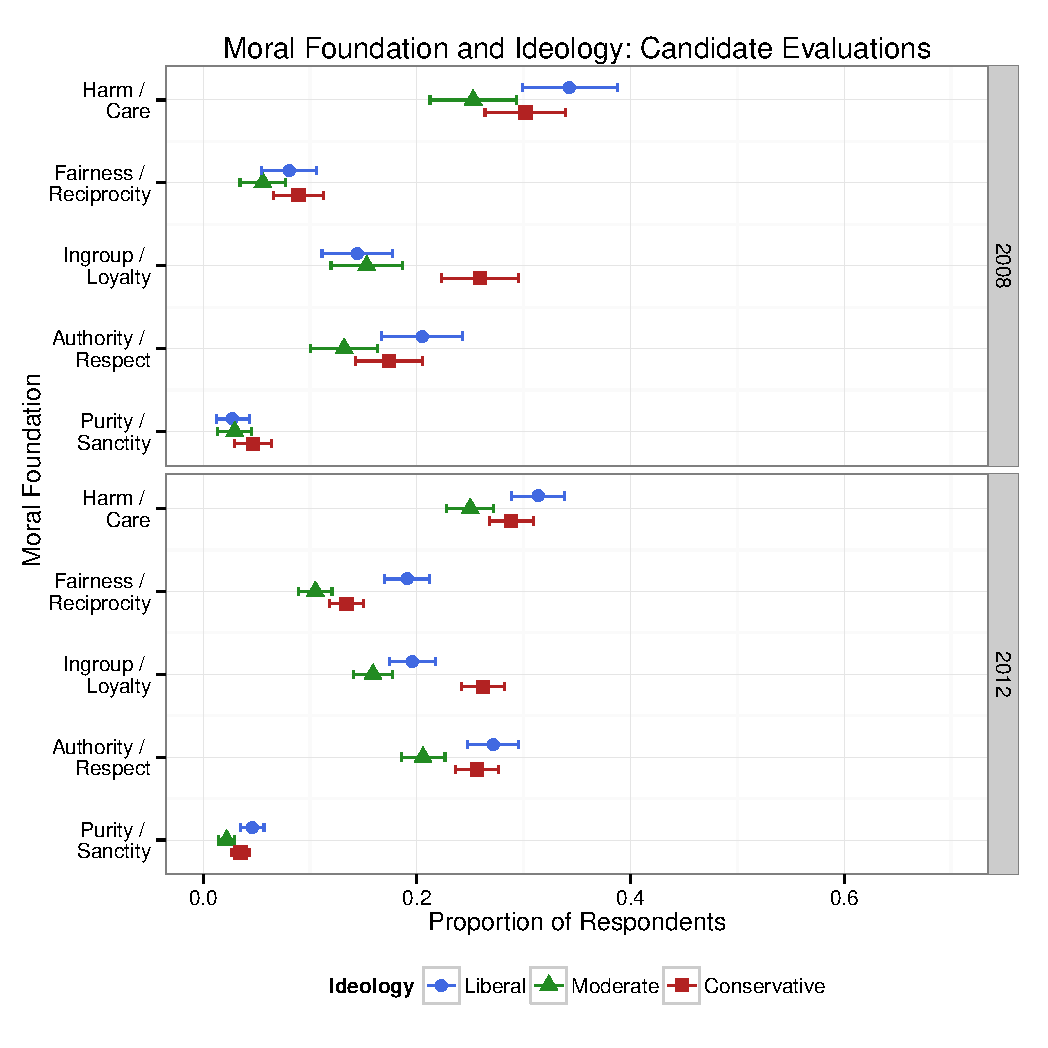
\includegraphics[scale=.6]{../calc/fig/p2_mft_ideol_ca.pdf}
\caption{Moral Foundations and Ideology (Party Evaluations)}\label{fig:mft_ideol_pa}
\end{figure}

\begin{figure}\centering
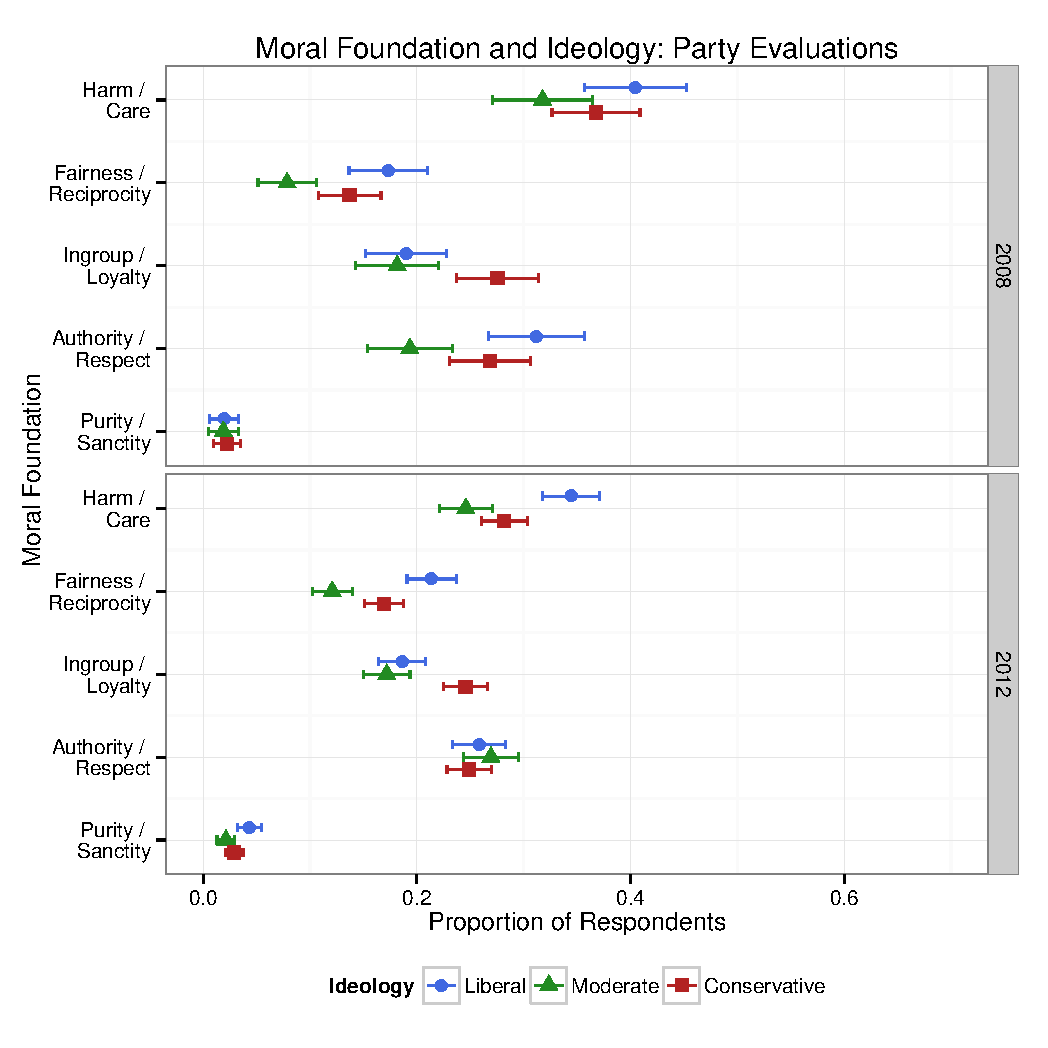
\includegraphics[scale=.6]{../calc/fig/p3_mft_ideol_pa.pdf}
\caption{Moral Foundations and Ideology (Candidate Evaluations)}\label{fig:mft_ideol_ca}
\end{figure}

Looking first at the results for 2012 (lower part of the plot), the patterns are largely consistent with our theoretical expectations. Liberals were most likely to mention the harm/care foundation. Slightly less than half of the respondents who identified as liberals mentioned words belonging to this category in their responses. Furthermore, they were more likely than conservatives to mention the fairness/reciprocity foundation. However, it should be noted that fairness/reciprocity was emphasized significantly less than the authority/respect foundation among liberals. Furthermore, conservatives were more likely to reference the ingroup/loyalty foundation. However, for the two remaining moral foundations, the patterns seem less clear. The proportion of liberal respondents referencing authority/respect is actually slightly larger than the proportion of conservatives (although not significant). This result is inconsistent with previous evidence in the moral foundations literature. Furthermore, the fact that the purity/sanctity foundation was almost never mentioned by any of the respondents is surprising, since other studies found that the purity/sanctity foundation plays a very important role when looking at ideological differences \citep{koleva2012tracing}. This result suggests that subsequent analyses of survey responses might necessitate a revision of the moral foundation dictionary, since the terms contained in the dictionary might not be relevant enough for political evaluations. Accordingly, some of the words (e.g. in the case of purity/sanctity) are just too uncommon in the political context. Due to the very rare mentioning of the purity/sanctity dimension, the subsequent analyses will only concentrate on the remaining four moral foundations.

Turning our attention to the results for 2008, it can be seen that the results that have been consistent with our expectations in 2012 (i.e. concerning the harm/care, fairness/reciprocity, and ingroup/loyalty dimensions) cannot be clearly replicated. Here the difference between liberals and conservatives is not significant except for the ingroup/loyalty foundation.

Instead of looking at the aggregation of all survey items, we can also investigate the patterns in smaller subsets of responses. Figure~\ref{fig:mft_ideol_pa} depicts the same proportions of references to moral foundations combining all open-ended responses related to the Republican and Democratic party. Figure~\ref{fig:mft_ideol_ca}, on the other hand, displays the equivalent results for the responses related to both presidential candidates. Instead of aggregating all responses for each individual, we now only combine items that asked for evaluations of parties \textit{or} candidates. Accordingly, the reported proportions indicate the percentage of respondents who referred to the respective moral foundation in any of their reported likes and dislikes for both candidates \textit{or} both parties.

The patterns are similar to the pooled analyses. For the 2012 survey, we see expected differences between liberals and conservatives in terms of the likelihood to emphasize moral foundations of harm/care, fairness/reciprocity, and ingroup/loyalty. However, for the two remaining dimensions (authority/respect), the difference is either marginal and/or inconsistent with the expectations of Moral Foundation Theory. Moreover, in 2008 ideological differences for all foundations except ingroup/loyalty become insignificant. However, it should be mentioned that the sample size of the 2008 ANES is much smaller, which explains the higher uncertainty about the estimated proportions. Overall, these results provide an inconclusive picture on the moral foundations of political reasoning. While some patterns are consistent with our theoretical expectations in 2012 (e.g. harm/care), they fail to be clearly replicated in 2008. The results discussed so far are similar if respondents are differentiated by partisanship rather than political ideology (see figures \ref{fig:a1_mft_pid}, \ref{fig:a2_mft_pid_ca}, and \ref{fig:a3_mft_pid_pa} in the Appendix).

In a subsequent step, I estimated logit models using ideology (and several control variables) to predict the individual probability to refer to either of the moral foundations (excluding purity/sanctity) in both surveys. Note that all models control for the total number of words used by each respondent for their open-ended responses.\footnote{The full logistic regression results are presented in the appendix, Table~\ref{tab:m1_mft}}. Figure~\ref{fig:m1_mft} displays the expected change in predicted probabilities to mention each moral foundation when comparing liberals and conservatives while holding all other variables constant at their respective means, along with 95\% confidence intervals. Again, equivalent to the discussion of Figure~\ref{fig:mft_ideol}, the responses for each individual were collapsed such that the dependent variables indicate whether any of their responses contained a reference to the moral foundations as identified by the dictionary. 

\begin{figure}\centering
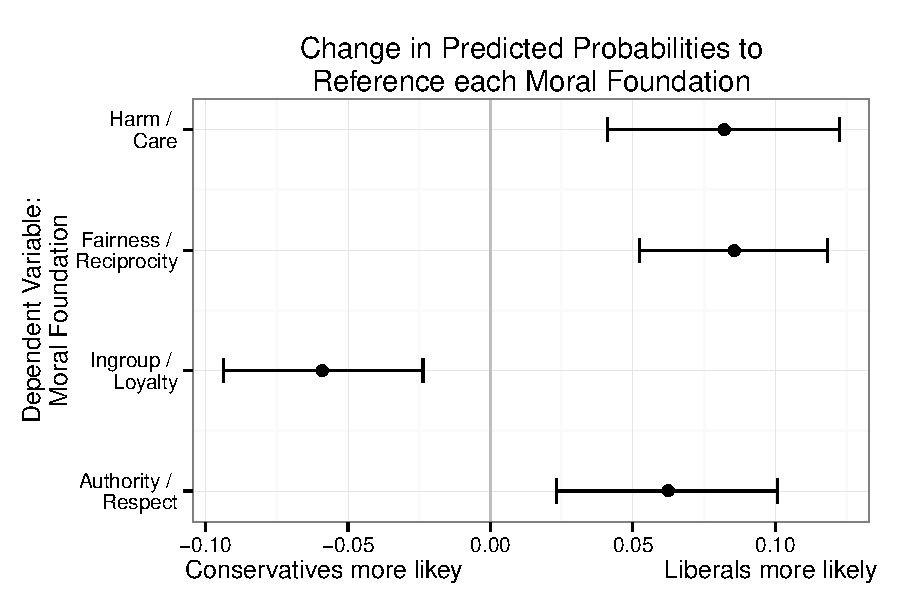
\includegraphics[scale=.6]{../calc/fig/m1_mft.pdf}
\caption{Difference in Predicted Probabilities to Reference each Moral Foundation between Liberals and Conservatives}\label{fig:m1_mft}
\end{figure}

Positive values indicate a higher probability to mention the respective moral foundation in a response among respondents who identified as liberals, while negative values indicate a higher probability among conservatives. In 2012, we find that the effects are consistent with our first hypothesis for three out of four moral foundations. Liberals are significantly more likely to mention harm/care and fairness/reciprocity when evaluating political parties and candidates than liberals. The probability to mention a word connected to the harm/care foundation is about 7.5 percentage points higher among liberals than conservatives. The effect is of similar size for the fairness/reciprocity dimension. Conversely, being conservative increases the likelihood of mentioning words that belong to the category of ingroup/loyalty by about 5 percentage points. However, liberals appear to be significantly more likely to reference the moral foundation of authority/respect when evaluating political actors. This result is inconsistent with previous evidence for the prevalence of authority/respect among conservatives. Furthermore, all other effects described above are not replicated when analyzing the 2008 ANES.

\begin{figure}\centering
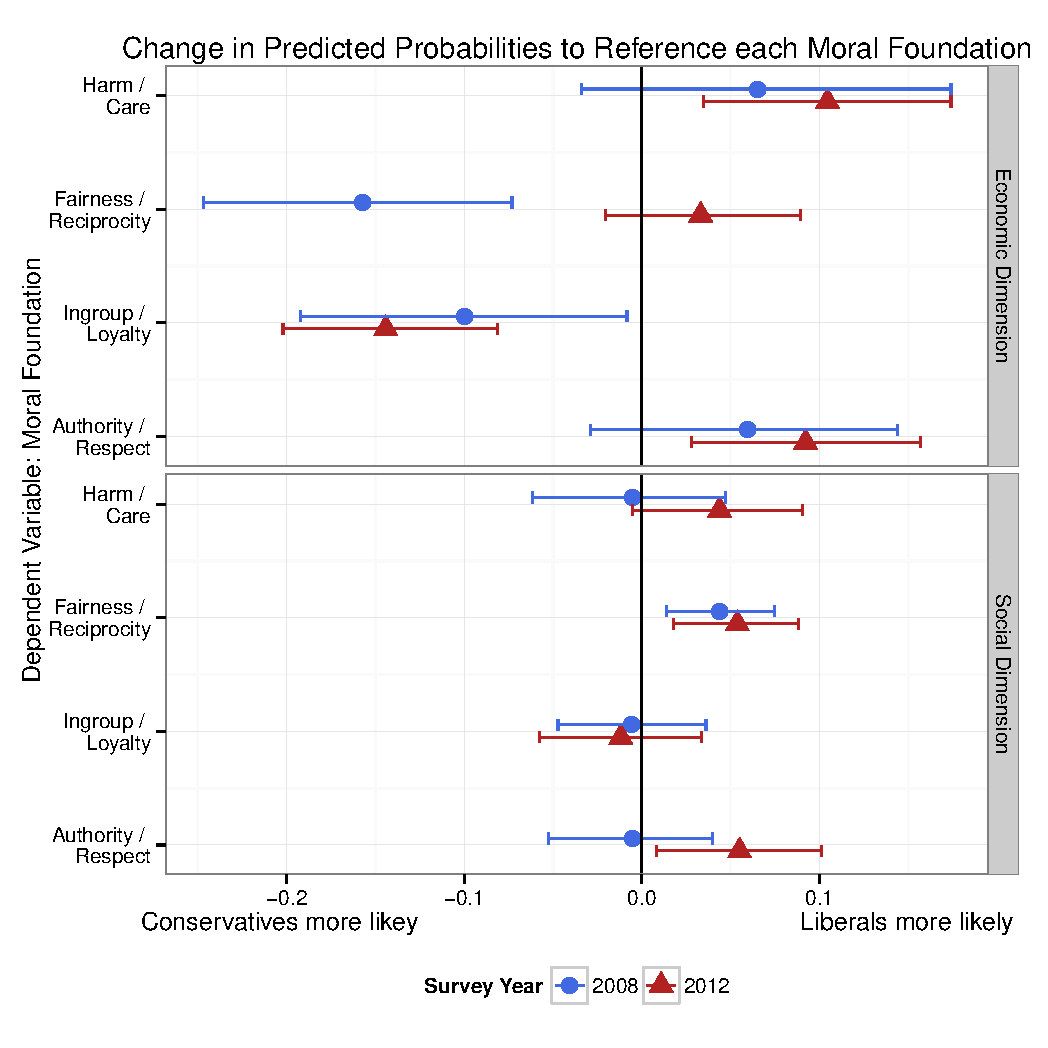
\includegraphics[scale=.6]{../calc/fig/m1b_mft.pdf}
\caption{Difference in Predicted Probabilities to Reference each Moral Foundation between Liberals and Conservatives on Economic and Social Dimension}\label{fig:m1b_mft}
\end{figure}

These inconsistencies could indicate that the unidimensional conceptualization of ideology, which has been used in most studies analyzing moral foundations theory, might be too simplistic in order to describe systematic differences between individuals who hold different political belief systems and ideologies. As such, I repeated the analyses using a conceptualization of ideology differentiating between a social as well as an economic dimension as proposed by \citet{feldman2013understanding}. The economic dimension is based on a summated scale containing items measuring issue preferences regarding increased government spending, public or private medical insurance, guaranteed jobs, and assistance to the poor. Social ideology, on the other hand, is measured by summarizing items on abortion, as well as gay adoption. Consistent with the results reported by \citet{feldman2013understanding}, exploratory factor analyses confirm that these items load on two independent dimensions (results not shown).\footnote{However, only a subset of these variables could be used for the ANES 2008, since the items on guaranteed jobs and abortion were not included for the entire sample.} The results are presented in Figure~\ref{fig:m1b_mft}.\footnote{The full logistic regression results are presented in the appendix, Table~\ref{tab:m1b_mft}} The figure displays the expected change in predicted probabilities to mention the respective moral foundation when comparing individuals who scored lowest on the ideological dimension (most conservative) to individuals who scored highest (most liberal), while holding all other variables constant at their respective means, along with 95\% confidence intervals.

Again, positive values indicate a higher probability to mention the respective moral foundation in a response among respondents who hold liberal attitudes on the ideological dimension, while negative values indicate a higher probability among conservatives. The results provide a more detailed picture than the previous analyses. Focusing first on 2012, individuals who hold liberal views on the economic dimension are more likely to mention harm/care considerations. Liberalism on the economic dimension did not have a significant effect on harm/care. This picture is reversed for fairness/reciprocity considerations. Here, liberal attitudes on the economic dimension had no effect, while social liberalism increased the probability to mention fairness/reciprocity. As such, it appears that considerations related to harm/care are driven by the economic dimension of political ideology and considerations related to fairness/reciprocity are driven by the social dimension. For the remaining foundations of ingroup/loyalty and authority/respect, the results for 2012 are similar to the unidimensional effects for both, economic as well as social liberalism. However, the results cannot be clearly replicated in 2008. While the effect of social liberalism on the likelihood to mention fairness/reciprocity is now significant and in the expected direction, most of the remaining effects are negligible. Furthermore, it appears that economic liberalism actually \textit{decreases} the likelihood to mention considerations related to the fairness/reciprocity foundation, which is a counter-intuitive result.

Instead of analyzing whether liberals or conservatives are more likely to emphasize either of the moral foundations, we can also investigate whether respondents, who mention specific moral considerations, are more likely to support the presidential candidates of either party. 

\begin{figure}[ht]\centering
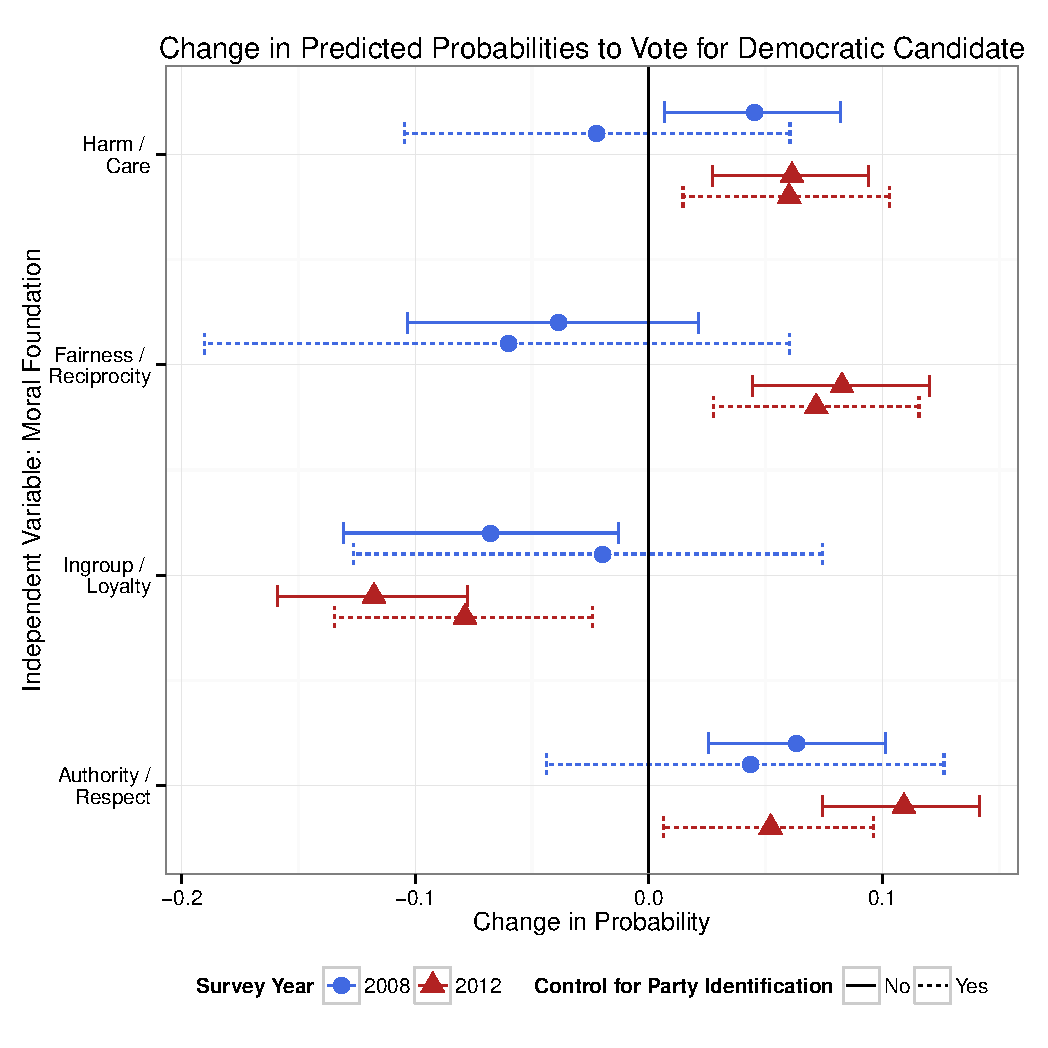
\includegraphics[scale=.6]{../calc/fig/m2_vote.pdf}
\caption{Change in Predicted Probabilities to Vote for Democratic Candidate Depending on References to Specific Moral Foundations}\label{fig:m2_vote}
\end{figure}

Figure~\ref{fig:m2_vote} presents the changes in expected probabilities to vote for the Democratic (vs. the Republican) presidential candidate in the 2008 and 2012 election if individuals used the respective moral foundations when evaluating both parties and candidates. The estimated probabilities are based on logit models including dummies for each moral foundation as independent variables as well as several sociodemographic control variables, which were held constant at their mean values when calculating expected values.\footnote{Full model results are displayed in the appendix, Table~\ref{tab:m2_vote}.}

While not all effects displayed in Figure~\ref{fig:m2_vote} are statistically significant (especially when looking at 2008), the patterns are quite similar to the results presented thus far. Individuals who mentioned moral considerations related to the harm/care foundation are (slightly) more likely to vote for the Democratic candidate. In 2012, the effect for the fairness/reciprocity foundation is also positive: respondents who mentioned this foundation were more likely to vote for Barack Obama than for Mitt Romney. For 2008, in contrast, the effects are negative and insignificant. Respondents who emphasized the ingroup/loyalty foundation, on the other hand, were less likely to vote for the Democratic candidate in both elections. While these results appear to be relatively consistent with Moral Foundations Theory, we see again that the effect for the authority/respect foundation deviates strikingly from our expectations: respondents mentioning this foundation were actually more likely to vote for the presidential candidate. This (as well as the previous) inconsistent result for the authority dimension could potentially be explained by the fact that many supporters of President Barack Obama described him as a good \textit{leader}, which is a signal word for the authority/respect dimension. Accordingly, it could be argued that the reliance on different moral considerations in political reasoning is (at least partly) context-specific.

It is worth emphasizing again that these effects do not differentiate whether individuals describe their preferred candidate or not. As such, the result shows that it is possible to predict voting behavior simply by observing the moral dimensions of the respondents' political reasoning, without taking into account which candidate they described, and whether the description is framed positively or negatively. As can be seen in the figure, most of these effects are even persistent when controlling for individual party identification.

The results discussed so far indicate that there are indeed important differences between liberals and conservatives in terms of their reliance on different moral considerations when evaluating political parties and candidates. However, the patterns cannot be described as unequivocally consistent with the predictions of Moral Foundations Theory. The fact that some foundations showed contrary patterns, as well as the failure to replicate some of the consistent 2012 findings in 2008 might suggest that the reliance on moral foundations might be more context-specific than the theorized innateness of moral intuitions would suggest.


\subsubsection{Determinants of Moral Reasoning}

After demonstrating that liberals and conservatives indeed differ with regard to the moral foundations they emphasize when evaluating political actors, we now turn to the question of whether the reliance on moral considerations in the domain of politics can be described as a product of exposure to political discourse.

I estimated logit models using political sophistication, political media exposure, and frequency of political discussions in order to predict the probability of individuals to mention \textit{any} moral foundation. Figure~\ref{fig:m3_learn} depicts the respective predicted probabilities when each independent variable (knowledge, media exposure, discussion) is increased from its empirical minimum value to its empirical maximum value, holding all other variables (including the number of words in each individual response) constant at their means.\footnote{Full model results are displayed in the appendix, Table~\ref{tab:m3_learn}.}

The results show, that most variables (except political discussions in 2008) have a positive effect on the individual probability to make use of moral foundations (in general) when evaluating political parties and candidates. Higher political sophistication, higher exposure to political media and news, as well as more frequent political discussions increase the probability that individuals rely on moral considerations. Thereby, citizens \textit{learn} to embed moral reasoning in their political evaluations. This argument should not be seen as refuting the argument of innateness of moral intuitions as described by Moral Foundation Theory. Moral intuitions themselves might well be innate. The extent to which individuals make use of these intuitions when thinking about politics and evaluating political actors appears to be more context-dependent and subject to individual heterogeneity.

\begin{figure}\centering
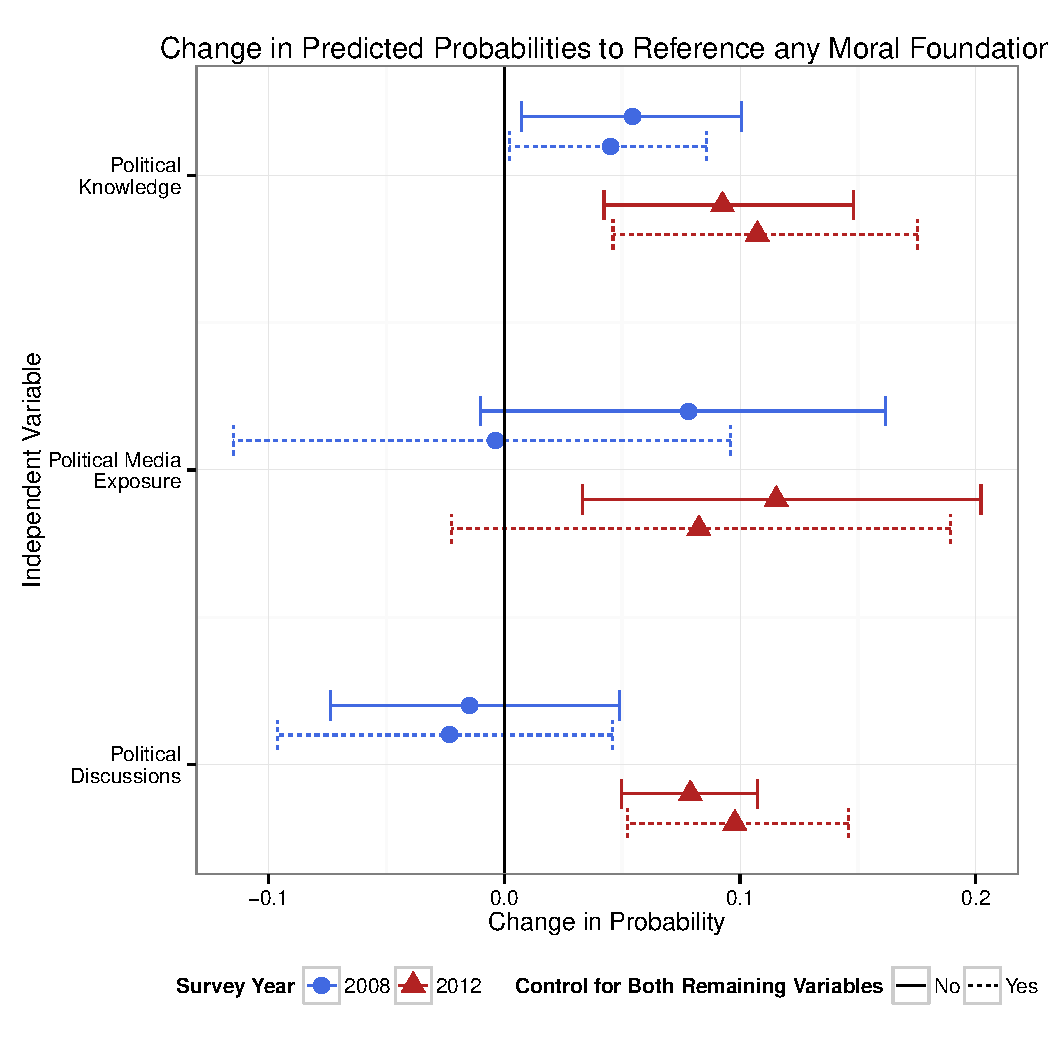
\includegraphics[scale=.6]{../calc/fig/m3_learn.pdf}
\caption{Change in Predicted Probabilities to Reference any of the Moral Foundations Depending on Political Knowledge, Media Exposure, and Frequency of Political Discussions}\label{fig:m3_learn}
\end{figure}

The significant positive effect of frequent political discussions in 2012 (even after controlling for the two remaining variables, political knowledge and media exposure), is especially interesting in this context. Citizens, who engage in frequent political arguments are more likely to use moral considerations when evaluating candidates and parties. This result could suggest that morality in politics plays an important role as a rhetorical tool utilized to convince others of certain political views.

The positive relationships between political knowledge, media exposure, and political discussions and moral reasoning appears to be quite robust, even when we control for overall individual response lengths. However, it should be noted that the analyses presented so far do not really allow us to make strong causal claims with regard to the political learning effects on moral reasoning. Further experimental research is necessary to investigate t

\section{Conclusion}

The goal of this paper was to investigate to what extent the ideological differences in the emphasis on moral foundations manifests itself in individual reasoning about political actors. It was argued that the analyses of open-ended survey responses can provide important insights beyond previous research because it allows to evaluate to what extent citizens make reference to moral considerations in a political context that does not induce an explicit connection to morality. Furthermore, it was argued that the reliance on moral reasoning as such is moderated by political knowledge, media exposure, and political discussions.

The empirical evidence discussed in this paper is only partly consistent with previous results on moral foundations and ideology. The first hypothesis, which predicted systematic patterns in the emphasis on moral considerations among liberals and conservatives was supported for three out of four foundations included in the analyses in one of the surveys. Liberals are more likely to mention considerations related to harm/care and fairness/reciprocity when discussing their political preferences, whereas conservatives are more likely to emphasize the moral foundation of ingroup/loyalty.

%%% ADD MORE STUFF HERE

According to the second hypothesis, it was expected that individuals show heterogeneity in terms of their tendency to rely on moral reasoning when evaluating political actors. The results showed that political knowledge, discussions, as well as media consumption increased the reliance on moral considerations. Thus, the evidence suggests that moral reasoning is part of a broader political learning process. It remains an open question, however, whether this learning process implies an increased differentiation between liberals and conservatives in terms of the focus on specific foundations as described by Moral Foundations Theory. The results presented here only show that moral reasoning becomes more prevalent with higher political involvement, but they are inconclusive as to whether learning process increase the ``moral differentiation'' of liberals and conservatives.
%
% Maybe I should add these analyses
%

Overall, the fact that purity/sanctity was almost never mentioned as well as the inconsistent effect of ideology on the authority/respect dimension could be attributed to the fact that the moral foundations dictionary was originally used for the analyses of sermons rather than in the context of day-to-day politics.\footnote{However, the collection of words used in \citet{graham2009liberals} was conceptualized as a general dictionary for multiple sources (see also \url{http://www.moralfoundations.org/})} Accordingly, subsequent analyses could revise the dictionary in order to make it more applicable for the analyses of survey responses. Furthermore, it should be noted that the modelling strategy based on multiple logistic regressions assumes independence between the different response categories. This assumptions does not seem to be plausible since the reference to a specific moral foundation might well affect how often individuals mention other considerations. While a multinomial logit / conditional logit framework is also not feasible due to the fact that individuals can fall in several categories, other model approaches for non-exclusive multinomial choices might allow to improve the empirical analyses \citep[see for example][]{gilbert2007models}.

An alternative approach to the analysis of open-ended survey responses could be the implementation of structural topic models as described by \citet{roberts2014structural}: instead of using explicit word lists to identify moral reasoning, it would possible to identify specific topics in open-ended responses that are consistent with the moral foundations described by \citet{haidt2008moral} \citep[see also][]{lin2008joint}.

Irrespective of these reservations and the resulting tentativeness of the empirical results presented thus far, the analyses of open-ended survey responses can provide important and valuable insights in the context of moral foundations and the individual underpinnings of political ideology. As such, there are numerous avenues for future research. For example, it would be interesting to investigate whether the reference to specific moral foundations differs between survey questions: Do individuals differ in terms of their moral considerations if they describe in-party or out-party candidates? Does the evaluations of parties and candidate elicit different considerations? Furthermore, are there sources of heterogeneity in moral foundations among liberals and conservatives? Utilizing available responses to open-ended survey questions provides a useful and still largely neglected data source to investigate these and other important research questions from novel perspectives.


\clearpage\flushleft\footnotesize\singlespacing
\appendices
\section{Moral Foundations Dictionary}
\renewcommand\thefigure{\thesection.\arabic{figure}}
\renewcommand\thetable{\thesection.\arabic{table}}
\setcounter{figure}{0}
\setcounter{table}{0}

\textit{Sources:}\\
\citet{graham2009liberals}, as well as \url{http://www.moralfoundations.org/}
\vspace{.5cm}

\textit{Note:}\\
Words with (*) indicate that the word stem rather than the exact word was matched in the open-ended survey responses.
\vspace{.5cm}

\textbf{Harm:}\\
safe*, peace*, compassion*, empath*, sympath*, care, caring, protect*, shield, shelter, amity, secur*, benefit*, defen*, guard*, preserve, harm*, suffer*, war, wars, warl*, warring, fight*, violen*, hurt*, kill, kills, killer*, killed, killing, endanger*, cruel*, brutal*, abuse*, damag*, ruin*, ravage, detriment*, crush*, attack*, annihilate*, destroy, stomp, abandon*, spurn, impair, exploit, exploits, exploited, exploiting, wound*
\vspace{.5cm}

\textbf{Fairness:}\\
fair, fairly, fairness, fair*, fairmind*, fairplay, equal*, justice, justness, justifi*, reciproc*, impartial*, egalitar*, rights, equity, evenness, equivalent, unbias*, tolerant, equable, balance*, homologous, unprejudice*, reasonable, constant, honest*, unfair*, unequal*, bias*, unjust*, injust*, bigot*, discriminat*, disproportion*, inequitable, prejud*, dishonest, unscrupulous, dissociate, preference, favoritism, segregat*, exclusion, exclud*
\vspace{.5cm}

\textbf{Ingroup:}\\
together, nation*, homeland*, family, families, familial, group, loyal*, patriot*, communal, commune*, communit*, communis*, comrad*, cadre, collectiv*, joint, unison, unite*, fellow*, guild, solidarity, devot*, member, cliqu*, cohort, ally, insider, foreign*, enem*, betray*, treason*, traitor*, treacher*, disloyal*, individual*, apostasy, apostate, deserted, deserter*, deserting, deceiv*, jilt*, imposter, miscreant, spy, sequester, renegade, terroris*, immigra*
\vspace{.5cm}

\textbf{Authority:}\\
obey*, obedien*, duty, law, lawful*, legal*, duti*, honor*, respect, respectful*, respected, respects, order*, father*, mother, motherl*, mothering, mothers, tradition*, hierarch*, authorit*, permit, permission, status*, rank*, leader*, class, bourgeoisie, caste*, position, complian*, command, supremacy, control, submi*, allegian*, serve, abide, defere*, defer, revere*, venerat*, comply, defian*, rebel*, dissent*, subver*, disrespect*, disobe*, sediti*, agitat*, insubordinat*, illegal*, lawless*, insurgent, mutinous, defy*, dissident, unfaithful, alienate, defector, heretic*, nonconformist, oppose, protest, refuse, denounce, remonstrate, riot*, obstruct
\vspace{.5cm}

\textbf{Purity:}\\
piety, pious, purity, pure*, clean*, steril*, sacred*, chast*, holy, holiness, saint*, wholesome*, celiba*, abstention, virgin, virgins, virginity, virginal, austerity, integrity, modesty, abstinen*, abstemiousness, upright, limpid, unadulterated, maiden, virtuous, refined, intemperate, decen*, immaculate, innocent, pristine, humble, disgust*, deprav*, disease*, unclean*, contagio*, indecen*, sin, sinful*, sinner*, sins, sinned, sinning, slut*, whore, dirt*, impiety, impious, profan*, gross, repuls*, sick*, promiscu*, lewd*, adulter*, debauche*, defile*, tramp, prostitut*, unchaste, wanton, profligate, filth*, trashy, obscen*, lax, taint*, stain*, tarnish*, debase*, desecrat*, wicked*, blemish, exploitat*, pervert, wretched*
\vspace{.5cm}

\textbf{General:}\\
righteous*, moral*, ethic*, value*, upstanding, good, goodness, principle*, blameless, exemplary, lesson, canon, doctrine, noble, worth*, ideal*, praiseworthy, commendable, character, proper, laudable, correct, wrong*, evil, immoral*, bad, offend*, offensive*, transgress*, honest*, lawful*, legal*, piety, pious, wholesome*, integrity, upright, decen*, indecen*, wicked*, wretched*


\clearpage
\section{Additional Tables and Figures - Overview}
\renewcommand\thefigure{\thesection.\arabic{figure}}
\renewcommand\thetable{\thesection.\arabic{table}}
\setcounter{figure}{0}
\setcounter{table}{0}

% latex table generated in R 3.2.2 by xtable 1.7-4 package
% Wed Sep 16 10:56:58 2015
\begin{table}[ht]
\centering
\begin{tabular}{lcc}
  \hline
 & N & Percent \\ 
  \hline
Spanish Interview (2008) & 94 & 4.05 \\ 
  Spanish Interview (2012) & 228 & 3.86 \\ 
  No Responses (Overall, 2008) & 158 & 7.09 \\ 
  No Responses (Overall, 2012) & 392 & 6.89 \\ 
  No Responses (Candidate Evaluations, 2008) & 328 & 14.13 \\ 
  No Responses (Candidate Evaluations, 2012) & 761 & 12.87 \\ 
  No Responses (Party Evaluations, 2008) & 584 & 25.15 \\ 
  No Responses (Party Evaluations, 2012) & 1503 & 25.41 \\ 
   \hline
\end{tabular}
\caption{Overview - Missing Open-Ended Responses} 
\label{tab:a1_mis}
\end{table}


\begin{figure}[ht]\centering
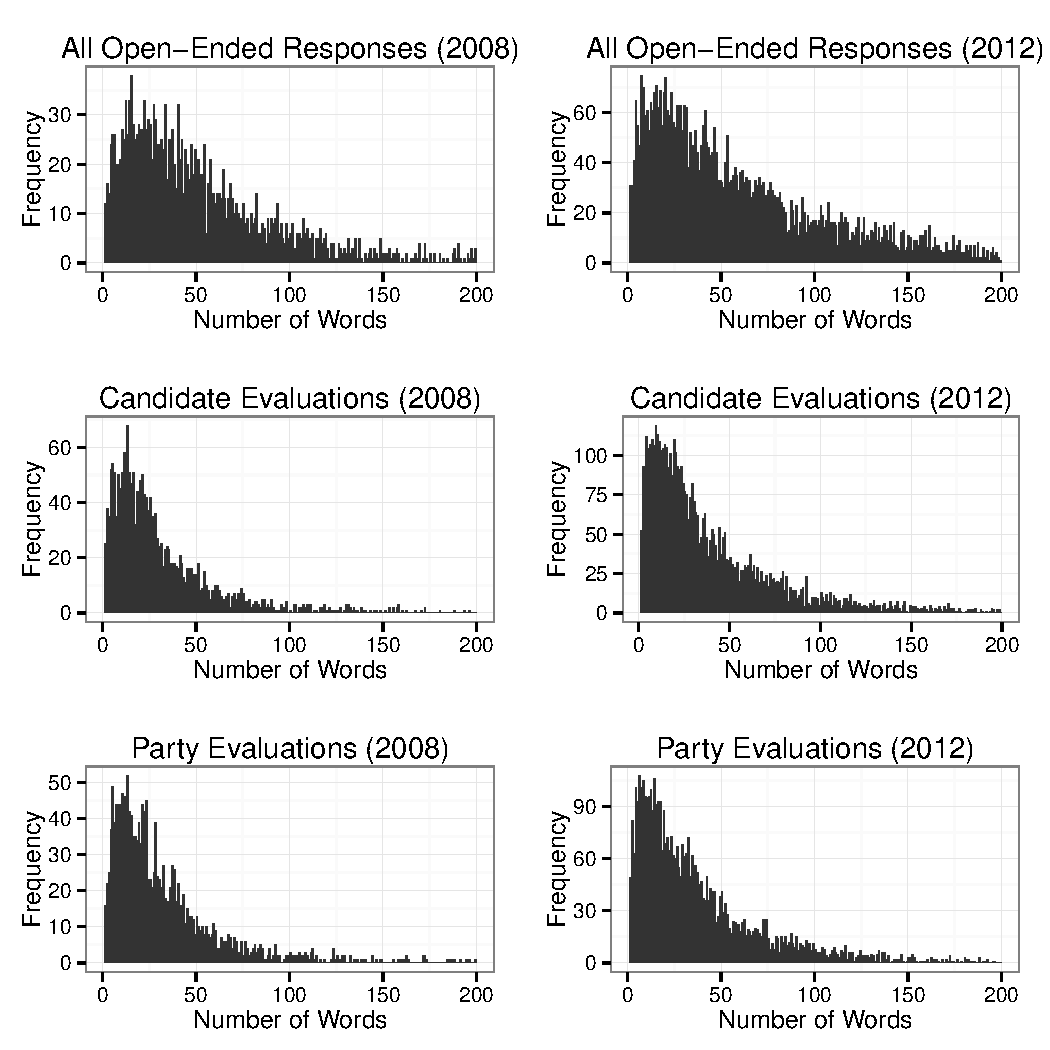
\includegraphics[scale=.8]{../calc/fig/a0_num.pdf}
\caption{Distribution of Numbers of Words in Open-Ended Responses}\label{fig:a0_num}
\end{figure}

\begin{figure}[ht]\centering
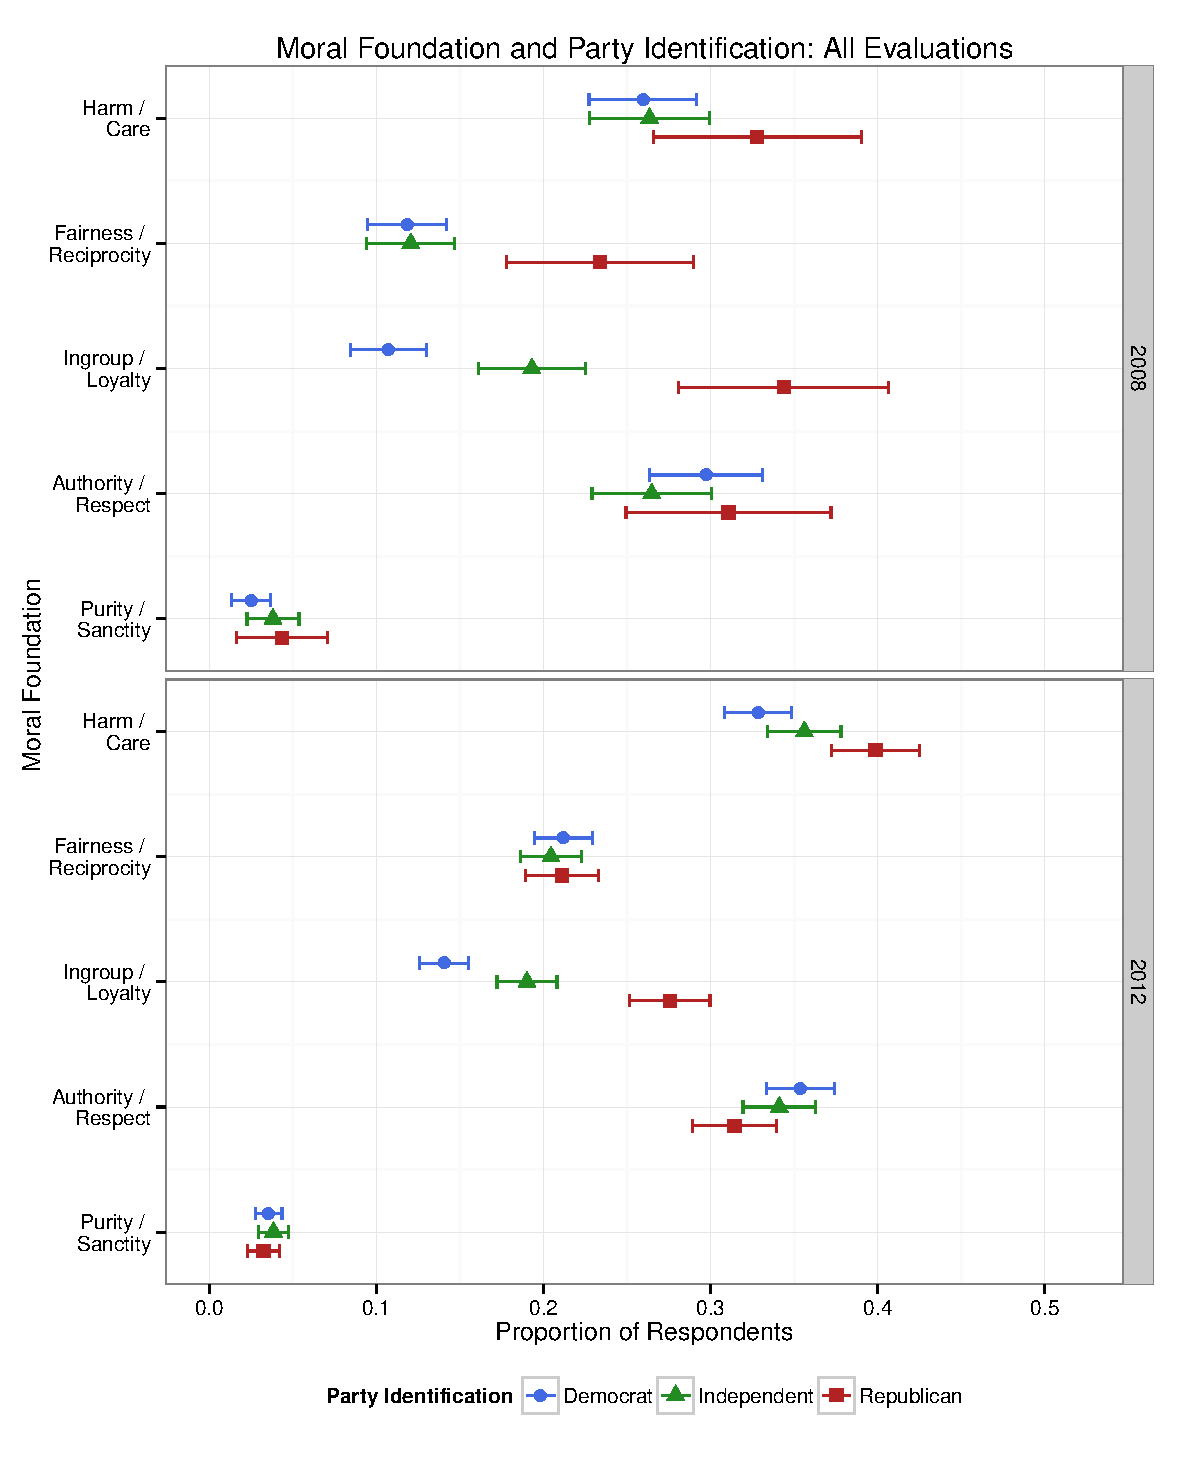
\includegraphics[scale=.4]{../calc/fig/a1_mft_pid.pdf}
\caption{Moral Foundations and Partisanship (all Statements)}\label{fig:a1_mft_pid}
\end{figure}

\begin{figure}[ht]\centering
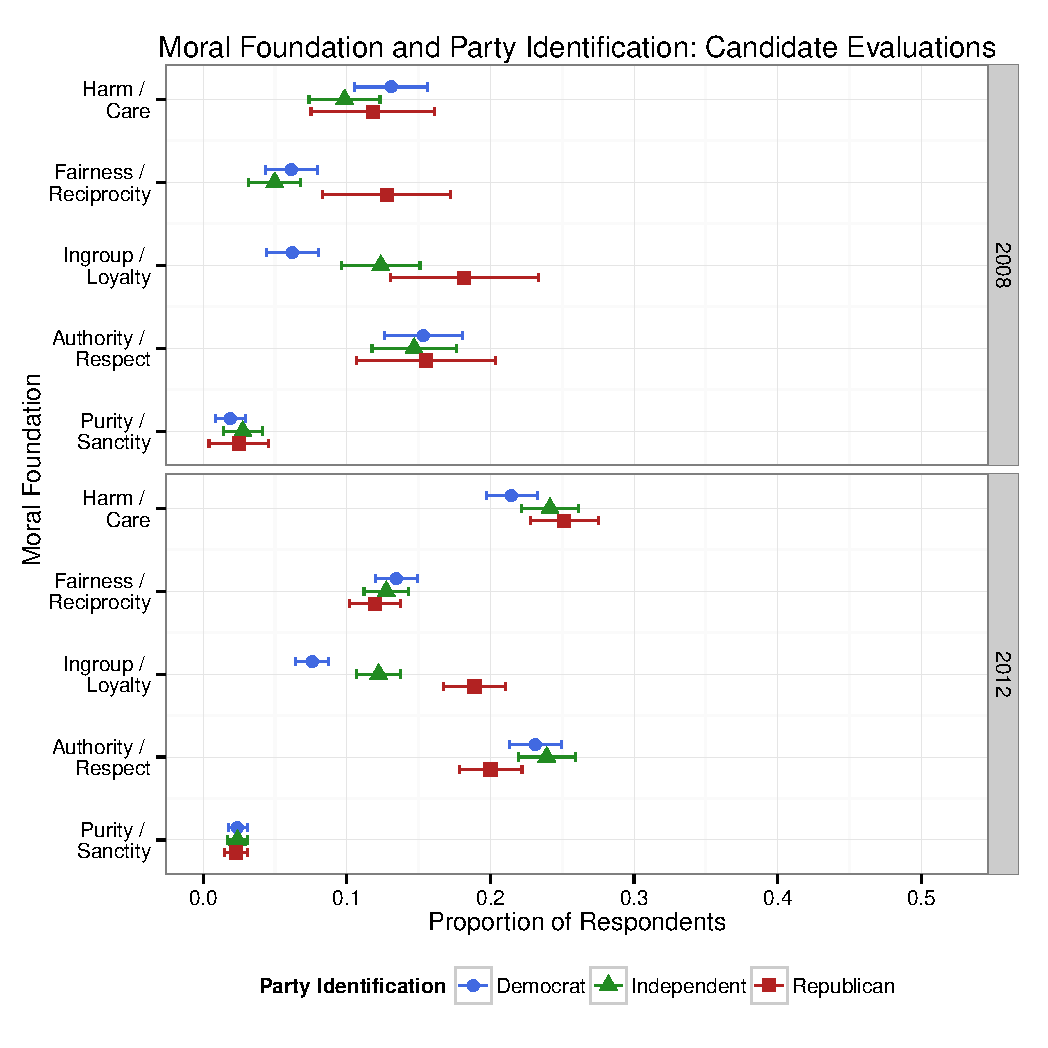
\includegraphics[scale=.4]{../calc/fig/a2_mft_pid_ca.pdf}
\caption{Moral Foundations and Partisanship (Candidate Evaluations)}\label{fig:a2_mft_pid_ca}
\end{figure}

\begin{figure}[ht]\centering
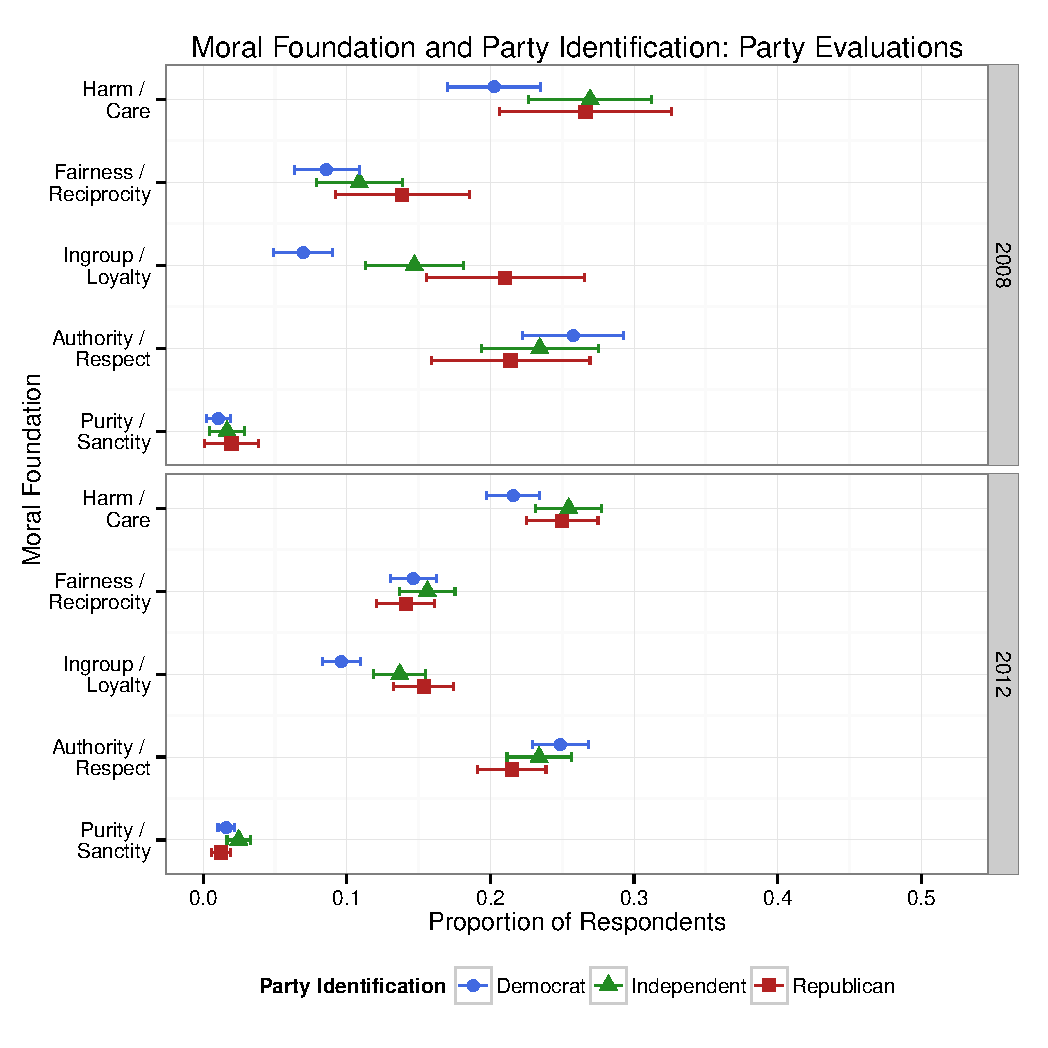
\includegraphics[scale=.4]{../calc/fig/a3_mft_pid_pa.pdf}
\caption{Moral Foundations and Partisanship (Party Evaluations)}\label{fig:a3_mft_pid_pa}
\end{figure}


\clearpage
\section{Tables of Logit Model Estimates}
\renewcommand\thefigure{\thesection.\arabic{figure}}
\renewcommand\thetable{\thesection.\arabic{table}}
\setcounter{figure}{0}
\setcounter{table}{0}


% Table created by stargazer v.5.2 by Marek Hlavac, Harvard University. E-mail: hlavac at fas.harvard.edu
% Date and time: Wed, Sep 16, 2015 - 10:57:06 AM
% Requires LaTeX packages: dcolumn 
\begin{table}[ht] \centering 
  \caption{Logit Models Predicting References to four Moral Foundations using Ideology} 
  \label{tab:m1_mft} 
\tiny 
\begin{tabular}{@{\extracolsep{-15pt}}lD{.}{.}{-3} D{.}{.}{-3} D{.}{.}{-3} D{.}{.}{-3} D{.}{.}{-3} D{.}{.}{-3} D{.}{.}{-3} D{.}{.}{-3} } 
\\[-1.8ex]\hline 
\hline \\[-1.8ex] 
 & \multicolumn{8}{c}{\textit{Dependent variable:}} \\ 
\cline{2-9} 
\\[-1.8ex] & \multicolumn{2}{c}{Harm / Care} & \multicolumn{2}{c}{Fairness / Reciprocity} & \multicolumn{2}{c}{Ingroup / Loyalty} & \multicolumn{2}{c}{Authority / Respect} \\ 
 & \multicolumn{1}{c}{2008} & \multicolumn{1}{c}{2012} & \multicolumn{1}{c}{2008} & \multicolumn{1}{c}{2012} & \multicolumn{1}{c}{2008} & \multicolumn{1}{c}{2012} & \multicolumn{1}{c}{2008} & \multicolumn{1}{c}{2012} \\ 
\hline \\[-1.8ex] 
 Conservative & -0.105 & -0.327^{***} & -0.005 & -0.440^{***} & 0.288 & 0.407^{***} & -0.342^{**} & -0.308^{***} \\ 
  & (0.160) & (0.084) & (0.198) & (0.093) & (0.192) & (0.104) & (0.153) & (0.085) \\ 
  Moderate & -0.144 & -0.383^{***} & -0.280 & -0.480^{***} & 0.158 & 0.133 & -0.442^{***} & -0.129 \\ 
  & (0.165) & (0.085) & (0.217) & (0.096) & (0.202) & (0.110) & (0.159) & (0.085) \\ 
  Church Attendance & -0.025 & -0.014 & -0.015 & 0.002 & 0.052 & 0.074^{***} & 0.064^{*} & -0.026 \\ 
  & (0.039) & (0.020) & (0.048) & (0.022) & (0.044) & (0.023) & (0.037) & (0.020) \\ 
  Education (College Degree) & 0.318^{**} & 0.032 & 0.306^{*} & 0.315^{***} & 0.458^{***} & 0.138^{*} & 0.321^{**} & 0.235^{***} \\ 
  & (0.140) & (0.070) & (0.182) & (0.077) & (0.171) & (0.083) & (0.134) & (0.070) \\ 
  Age & -0.017^{***} & -0.004^{**} & 0.010^{**} & 0.003 & 0.001 & 0.002 & -0.004 & 0.008^{***} \\ 
  & (0.004) & (0.002) & (0.005) & (0.002) & (0.005) & (0.002) & (0.004) & (0.002) \\ 
  Sex (Female) & 0.074 & 0.274^{***} & 0.154 & 0.133^{*} & -0.085 & -0.007 & -0.182 & -0.069 \\ 
  & (0.129) & (0.067) & (0.164) & (0.076) & (0.152) & (0.081) & (0.124) & (0.067) \\ 
  Race (African American) & -0.044 & -0.028 & -0.102 & -0.139 & 0.235 & 0.012 & -0.071 & 0.417^{***} \\ 
  & (0.166) & (0.092) & (0.219) & (0.108) & (0.191) & (0.114) & (0.160) & (0.091) \\ 
  Number of Words & 0.013^{***} & 0.011^{***} & 0.008^{***} & 0.008^{***} & 0.011^{***} & 0.011^{***} & 0.010^{***} & 0.012^{***} \\ 
  & (0.001) & (0.001) & (0.001) & (0.0005) & (0.001) & (0.001) & (0.001) & (0.001) \\ 
  Constant & -1.193^{***} & -1.108^{***} & -3.164^{***} & -1.935^{***} & -3.062^{***} & -2.839^{***} & -1.362^{***} & -1.811^{***} \\ 
  & (0.249) & (0.126) & (0.335) & (0.144) & (0.315) & (0.163) & (0.241) & (0.132) \\ 
 \hline \\[-1.8ex] 
Observations & \multicolumn{1}{c}{1,468} & \multicolumn{1}{c}{4,691} & \multicolumn{1}{c}{1,468} & \multicolumn{1}{c}{4,691} & \multicolumn{1}{c}{1,468} & \multicolumn{1}{c}{4,691} & \multicolumn{1}{c}{1,468} & \multicolumn{1}{c}{4,691} \\ 
Log Likelihood & \multicolumn{1}{c}{-754.236} & \multicolumn{1}{c}{-2,718.587} & \multicolumn{1}{c}{-528.080} & \multicolumn{1}{c}{-2,251.633} & \multicolumn{1}{c}{-586.828} & \multicolumn{1}{c}{-2,015.282} & \multicolumn{1}{c}{-802.048} & \multicolumn{1}{c}{-2,684.276} \\ 
Akaike Inf. Crit. & \multicolumn{1}{c}{1,526.472} & \multicolumn{1}{c}{5,455.174} & \multicolumn{1}{c}{1,074.159} & \multicolumn{1}{c}{4,521.265} & \multicolumn{1}{c}{1,191.656} & \multicolumn{1}{c}{4,048.565} & \multicolumn{1}{c}{1,622.097} & \multicolumn{1}{c}{5,386.553} \\ 
\hline 
\hline \\[-1.8ex] 
\textit{Note:}  & \multicolumn{8}{r}{$^{*}$p$<$0.1; $^{**}$p$<$0.05; $^{***}$p$<$0.01} \\ 
\end{tabular} 
\end{table} 



% Table created by stargazer v.5.2 by Marek Hlavac, Harvard University. E-mail: hlavac at fas.harvard.edu
% Date and time: Wed, Sep 16, 2015 - 03:50:00 PM
% Requires LaTeX packages: dcolumn 
\begin{table}[ht] \centering 
  \caption{Logit Models Predicting References to four Moral Foundations using Two-dimensional Conceptualization of Ideology} 
  \label{tab:m1b_mft} 
\tiny 
\begin{tabular}{@{\extracolsep{-15pt}}lD{.}{.}{-3} D{.}{.}{-3} D{.}{.}{-3} D{.}{.}{-3} D{.}{.}{-3} D{.}{.}{-3} D{.}{.}{-3} D{.}{.}{-3} } 
\\[-1.8ex]\hline 
\hline \\[-1.8ex] 
 & \multicolumn{8}{c}{\textit{Dependent variable:}} \\ 
\cline{2-9} 
\\[-1.8ex] & \multicolumn{2}{c}{Harm / Care} & \multicolumn{2}{c}{Fairness / Reciprocity} & \multicolumn{2}{c}{Ingroup / Loyalty} & \multicolumn{2}{c}{Authority / Respect} \\ 
 & \multicolumn{1}{c}{2008} & \multicolumn{1}{c}{2012} & \multicolumn{1}{c}{2008} & \multicolumn{1}{c}{2012} & \multicolumn{1}{c}{2008} & \multicolumn{1}{c}{2012} & \multicolumn{1}{c}{2008} & \multicolumn{1}{c}{2012} \\ 
\hline \\[-1.8ex] 
 Economic Liberalism & 0.127 & 0.452^{***} & -1.205^{***} & 0.161 & 0.089 & -0.375^{**} & 0.456^{*} & 0.491^{***} \\ 
  & (0.252) & (0.146) & (0.312) & (0.165) & (0.301) & (0.177) & (0.245) & (0.148) \\ 
  Social Liberalism & -0.053 & 0.148 & 0.478^{***} & 0.347^{***} & -0.098 & -0.312^{**} & 0.002 & 0.289^{***} \\ 
  & (0.126) & (0.105) & (0.165) & (0.123) & (0.153) & (0.128) & (0.121) & (0.107) \\ 
  Moderate & -0.020 & -0.008 & 0.020 & 0.015 & 0.047 & 0.056^{**} & 0.047 & -0.005 \\ 
  & (0.035) & (0.020) & (0.044) & (0.023) & (0.041) & (0.024) & (0.033) & (0.021) \\ 
  Church Attendance & 0.222^{*} & 0.086 & 0.171 & 0.374^{***} & 0.376^{**} & 0.187^{**} & 0.359^{***} & 0.215^{***} \\ 
  & (0.121) & (0.070) & (0.161) & (0.077) & (0.150) & (0.084) & (0.118) & (0.070) \\ 
  Education (College Degree) & -0.012^{***} & -0.003 & 0.013^{***} & 0.003 & -0.002 & 0.003 & -0.007^{*} & 0.006^{***} \\ 
  & (0.004) & (0.002) & (0.005) & (0.002) & (0.004) & (0.002) & (0.003) & (0.002) \\ 
  Age & 0.167 & 0.280^{***} & 0.218 & 0.117 & -0.182 & -0.054 & -0.111 & -0.102 \\ 
  & (0.118) & (0.065) & (0.154) & (0.074) & (0.142) & (0.080) & (0.114) & (0.066) \\ 
  Sex (Female) & -0.062 & -0.004 & 0.051 & -0.184^{*} & 0.138 & 0.056 & -0.128 & 0.391^{***} \\ 
  & (0.138) & (0.088) & (0.186) & (0.105) & (0.164) & (0.111) & (0.134) & (0.088) \\ 
  Race (African American) & 0.013^{***} & 0.011^{***} & 0.009^{***} & 0.008^{***} & 0.012^{***} & 0.011^{***} & 0.012^{***} & 0.012^{***} \\ 
  & (0.001) & (0.001) & (0.001) & (0.0005) & (0.001) & (0.001) & (0.001) & (0.001) \\ 
  Number of Words & -1.618^{***} & -1.797^{***} & -3.005^{***} & -2.643^{***} & -2.763^{***} & -2.311^{***} & -1.966^{***} & -2.343^{***} \\ 
  & (0.282) & (0.151) & (0.368) & (0.175) & (0.346) & (0.182) & (0.275) & (0.156) \\ 
 \hline \\[-1.8ex] 
Observations & \multicolumn{1}{c}{1,908} & \multicolumn{1}{c}{4,970} & \multicolumn{1}{c}{1,908} & \multicolumn{1}{c}{4,970} & \multicolumn{1}{c}{1,908} & \multicolumn{1}{c}{4,970} & \multicolumn{1}{c}{1,908} & \multicolumn{1}{c}{4,970} \\ 
Log Likelihood & \multicolumn{1}{c}{-950.669} & \multicolumn{1}{c}{-2,884.275} & \multicolumn{1}{c}{-633.070} & \multicolumn{1}{c}{-2,355.644} & \multicolumn{1}{c}{-708.579} & \multicolumn{1}{c}{-2,112.229} & \multicolumn{1}{c}{-1,000.887} & \multicolumn{1}{c}{-2,839.476} \\ 
Akaike Inf. Crit. & \multicolumn{1}{c}{1,919.338} & \multicolumn{1}{c}{5,786.549} & \multicolumn{1}{c}{1,284.141} & \multicolumn{1}{c}{4,729.288} & \multicolumn{1}{c}{1,435.159} & \multicolumn{1}{c}{4,242.458} & \multicolumn{1}{c}{2,019.775} & \multicolumn{1}{c}{5,696.953} \\ 
\hline 
\hline \\[-1.8ex] 
\textit{Note:}  & \multicolumn{8}{r}{$^{*}$p$<$0.1; $^{**}$p$<$0.05; $^{***}$p$<$0.01} \\ 
\end{tabular} 
\end{table} 



% Table created by stargazer v.5.2 by Marek Hlavac, Harvard University. E-mail: hlavac at fas.harvard.edu
% Date and time: Tue, Nov 10, 2015 - 12:11:17 PM
% Requires LaTeX packages: dcolumn 
\begin{table}[ht] \centering 
  \caption{Logit Models Predicting Democratic Vote Choice Based on Moral Foundations} 
  \label{tab:m2_vote} 
\tiny 
\begin{tabular}{@{\extracolsep{-15pt}}lD{.}{.}{-3} D{.}{.}{-3} D{.}{.}{-3} D{.}{.}{-3} } 
\\[-1.8ex]\hline 
\hline \\[-1.8ex] 
 & \multicolumn{4}{c}{\textit{Dependent variable:}} \\ 
\cline{2-5} 
\\[-1.8ex] & \multicolumn{4}{c}{Vote for Democratic Presidential Candidate} \\ 
 & \multicolumn{2}{c}{2008} & \multicolumn{2}{c}{2012} \\ 
\\[-1.8ex] & \multicolumn{1}{c}{(1)} & \multicolumn{1}{c}{(2)} & \multicolumn{1}{c}{(3)} & \multicolumn{1}{c}{(4)}\\ 
\hline \\[-1.8ex] 
 Harm / Care & 0.292^{**} & -0.099 & 0.270^{***} & 0.286^{***} \\ 
  & (0.122) & (0.183) & (0.079) & (0.111) \\ 
  Fairness / Reciprocity & -0.207 & -0.245 & 0.376^{***} & 0.344^{***} \\ 
  & (0.167) & (0.273) & (0.090) & (0.124) \\ 
  Ingroup / Loyalty & -0.348^{**} & -0.087 & -0.481^{***} & -0.341^{***} \\ 
  & (0.140) & (0.214) & (0.086) & (0.118) \\ 
  Authority / Respect & 0.408^{***} & 0.209 & 0.507^{***} & 0.245^{**} \\ 
  & (0.132) & (0.200) & (0.081) & (0.111) \\ 
  Party Identification (Democrat) &  & 2.888^{***} &  & 2.592^{***} \\ 
  &  & (0.183) &  & (0.131) \\ 
  Party Identification (Republican) &  & -2.260^{***} &  & -2.560^{***} \\ 
  &  & (0.411) &  & (0.143) \\ 
  Church Attendance & -0.226^{***} & -0.099^{*} & -0.311^{***} & -0.274^{***} \\ 
  & (0.033) & (0.051) & (0.022) & (0.030) \\ 
  Education (College Degree) & -0.362^{***} & -0.343^{*} & 0.077 & 0.213^{**} \\ 
  & (0.121) & (0.177) & (0.079) & (0.108) \\ 
  Age & -0.017^{***} & -0.030^{***} & -0.014^{***} & -0.022^{***} \\ 
  & (0.003) & (0.005) & (0.002) & (0.003) \\ 
  Sex (Female) & 0.388^{***} & 0.101 & 0.365^{***} & 0.306^{***} \\ 
  & (0.117) & (0.172) & (0.075) & (0.103) \\ 
  Race (African American) & 4.330^{***} & 3.693^{***} & 3.974^{***} & 3.056^{***} \\ 
  & (0.390) & (0.468) & (0.229) & (0.256) \\ 
  Constant & 1.269^{***} & 0.592^{**} & 0.743^{***} & 1.007^{***} \\ 
  & (0.207) & (0.291) & (0.136) & (0.190) \\ 
 \hline \\[-1.8ex] 
Observations & \multicolumn{1}{c}{1,822} & \multicolumn{1}{c}{1,313} & \multicolumn{1}{c}{3,973} & \multicolumn{1}{c}{3,963} \\ 
Log Likelihood & \multicolumn{1}{c}{-886.197} & \multicolumn{1}{c}{-453.056} & \multicolumn{1}{c}{-2,096.122} & \multicolumn{1}{c}{-1,237.334} \\ 
Akaike Inf. Crit. & \multicolumn{1}{c}{1,792.393} & \multicolumn{1}{c}{930.112} & \multicolumn{1}{c}{4,212.244} & \multicolumn{1}{c}{2,498.669} \\ 
\hline 
\hline \\[-1.8ex] 
\textit{Note:}  & \multicolumn{4}{r}{$^{*}$p$<$0.1; $^{**}$p$<$0.05; $^{***}$p$<$0.01} \\ 
\end{tabular} 
\end{table} 



% Table created by stargazer v.5.1 by Marek Hlavac, Harvard University. E-mail: hlavac at fas.harvard.edu
% Date and time: Sun, Dec 14, 2014 - 03:16:26 PM
% Requires LaTeX packages: dcolumn 
\begin{table}[ht] \centering 
  \caption{Logit Models Predicting Overall References to Moral Foundations} 
  \label{tab:m3_learn} 
\tiny 
\begin{tabular}{@{\extracolsep{-15pt}}lD{.}{.}{-3} D{.}{.}{-3} D{.}{.}{-3} D{.}{.}{-3} D{.}{.}{-3} D{.}{.}{-3} D{.}{.}{-3} D{.}{.}{-3} } 
\\[-1.8ex]\hline 
\hline \\[-1.8ex] 
 & \multicolumn{8}{c}{\textit{Dependent variable:}} \\ 
\cline{2-9} 
\\[-1.8ex] & \multicolumn{8}{c}{Reference to any Moral Foundation} \\ 
 & \multicolumn{1}{c}{2008} & \multicolumn{1}{c}{2012} & \multicolumn{1}{c}{2008} & \multicolumn{1}{c}{2012} & \multicolumn{1}{c}{2008} & \multicolumn{1}{c}{2012} & \multicolumn{1}{c}{2008} & \multicolumn{1}{c}{2012} \\ 
\\[-1.8ex] & \multicolumn{1}{c}{(1)} & \multicolumn{1}{c}{(2)} & \multicolumn{1}{c}{(3)} & \multicolumn{1}{c}{(4)} & \multicolumn{1}{c}{(5)} & \multicolumn{1}{c}{(6)} & \multicolumn{1}{c}{(7)} & \multicolumn{1}{c}{(8)}\\ 
\hline \\[-1.8ex] 
 Political Knowledge & 0.261^{**} & 0.149^{***} &  &  &  &  & 0.219^{*} & 0.142^{***} \\ 
  & (0.117) & (0.033) &  &  &  &  & (0.125) & (0.035) \\ 
  Political Media Exposure &  &  & 0.027^{***} & 0.019^{***} &  &  & 0.017^{*} & 0.011^{*} \\ 
  &  &  & (0.009) & (0.006) &  &  & (0.010) & (0.006) \\ 
  Political Discussions &  &  &  &  & 0.001 & 0.091^{***} & -0.011 & 0.079^{***} \\ 
  &  &  &  &  & (0.025) & (0.019) & (0.026) & (0.019) \\ 
  Church Attendance & 0.022 & -0.020 & 0.022 & -0.020 & 0.013 & -0.018 & 0.012 & -0.019 \\ 
  & (0.031) & (0.019) & (0.030) & (0.019) & (0.033) & (0.020) & (0.033) & (0.020) \\ 
  Education (College Degree) & 0.379^{***} & 0.185^{**} & 0.442^{***} & 0.239^{***} & 0.480^{***} & 0.282^{***} & 0.402^{***} & 0.183^{**} \\ 
  & (0.114) & (0.077) & (0.106) & (0.075) & (0.116) & (0.077) & (0.121) & (0.081) \\ 
  Age & -0.005 & -0.002 & -0.008^{**} & -0.003 & -0.003 & 0.0002 & -0.004 & -0.003 \\ 
  & (0.003) & (0.002) & (0.003) & (0.002) & (0.003) & (0.002) & (0.004) & (0.002) \\ 
  Sex (Female) & -0.094 & 0.226^{***} & -0.064 & 0.204^{***} & -0.135 & 0.195^{***} & -0.123 & 0.243^{***} \\ 
  & (0.109) & (0.068) & (0.104) & (0.067) & (0.114) & (0.069) & (0.115) & (0.071) \\ 
  Race (African American) & -0.057 & 0.445^{***} & -0.096 & 0.367^{***} & -0.070 & 0.358^{***} & -0.023 & 0.418^{***} \\ 
  & (0.127) & (0.091) & (0.118) & (0.088) & (0.133) & (0.092) & (0.135) & (0.094) \\ 
  Number of Words & 0.029^{***} & 0.025^{***} & 0.029^{***} & 0.026^{***} & 0.028^{***} & 0.025^{***} & 0.027^{***} & 0.025^{***} \\ 
  & (0.002) & (0.001) & (0.002) & (0.001) & (0.002) & (0.001) & (0.002) & (0.001) \\ 
  Constant & -1.411^{***} & -1.319^{***} & -1.481^{***} & -1.067^{***} & -1.274^{***} & -1.066^{***} & -1.484^{***} & -1.464^{***} \\ 
  & (0.201) & (0.143) & (0.195) & (0.122) & (0.209) & (0.124) & (0.227) & (0.152) \\ 
 \hline \\[-1.8ex] 
Observations & \multicolumn{1}{c}{1,845} & \multicolumn{1}{c}{5,147} & \multicolumn{1}{c}{2,031} & \multicolumn{1}{c}{5,177} & \multicolumn{1}{c}{1,648} & \multicolumn{1}{c}{4,842} & \multicolumn{1}{c}{1,646} & \multicolumn{1}{c}{4,807} \\ 
Log Likelihood & \multicolumn{1}{c}{-1,016.596} & \multicolumn{1}{c}{-2,670.308} & \multicolumn{1}{c}{-1,118.869} & \multicolumn{1}{c}{-2,689.725} & \multicolumn{1}{c}{-915.937} & \multicolumn{1}{c}{-2,495.047} & \multicolumn{1}{c}{-912.088} & \multicolumn{1}{c}{-2,467.724} \\ 
Akaike Inf. Crit. & \multicolumn{1}{c}{2,049.192} & \multicolumn{1}{c}{5,356.616} & \multicolumn{1}{c}{2,253.737} & \multicolumn{1}{c}{5,395.450} & \multicolumn{1}{c}{1,847.874} & \multicolumn{1}{c}{5,006.093} & \multicolumn{1}{c}{1,844.175} & \multicolumn{1}{c}{4,955.448} \\ 
\hline 
\hline \\[-1.8ex] 
\textit{Note:}  & \multicolumn{8}{r}{$^{*}$p$<$0.1; $^{**}$p$<$0.05; $^{***}$p$<$0.01} \\ 
\end{tabular} 
\end{table} 


\clearpage
\bibliographystyle{/data/Copy/1-src/lit/apsr2006}
\bibliography{/data/Copy/1-src/lit/Literature}
\end{document}